\documentclass[review,sort&compress]{elsarticle}
%%\usepackage{lgrind}

%\usepackage[square,comma,numbers,sort&compress]{natbib}
\usepackage{amsmath,amsthm,amssymb,amsfonts,amsbsy,latexsym} %amsthm inclusion conflicts with sisc...
%\usepackage{amsmath,amssymb,amsfonts,amsbsy,latexsym}
\usepackage{graphics}
%\usepackage{epsfig}
%%\usepackage[hang,raggedright]{subfigure}
%\usepackage{epsf}
%\usepackage{setspace}
%\usepackage{hangcaption}
\usepackage{graphicx}    % needed for including graphics e.g. EPS, PS
\usepackage{multirow}
%\usepackage{threeparttable}
\usepackage{cancel}
\usepackage{enumerate}
\usepackage{color}
\usepackage{hyperref}
\usepackage{cleveref}

\usepackage{algorithmicx}
\usepackage[ruled]{algorithm}
\usepackage{algpseudocode}
\usepackage{varwidth}
%\usepackage{caption}
%\usepackage[font=small]{subcaption}
%\usepackage{longtable}
\usepackage{mathrsfs}
\usepackage{upgreek}
\usepackage[caption=false]{subfig} % for \subfloat

\usepackage{lineno} %line numbering

\hypersetup{
    colorlinks=true,       % false: boxed links; true: colored links
    linkcolor=black,          % color of internal links
    citecolor=black,        % color of links to bibliography
    filecolor=magenta,      % color of file links
    urlcolor=blue           % color of external links
}

\newcommand{\R}{{\mathbb{R}}}
\newcommand{\Reals}{{\mathbb{R}}}
\newcommand{\bit}{\begin{itemize}}
\newcommand{\eit}{\end{itemize}}
\newcommand{\red}[1]{{\color{red}{#1}}}
\newcommand{\orderof}[1]{{\ensuremath{ {\cal O}(#1)}}}

\newtheorem{theorem}{Theorem}
\newtheorem{proposition}{Proposition}

\graphicspath{{./figures/}}

\begin{document}
%\raggedbottom %avoid weird vertical justification

\begin{frontmatter}

\title{Model Adaptivity for Goal-Oriented Inference using Adjoints}

%\author{Harriet Li\textsuperscript{a,}\footnote{Corresponding author. \textit{Email address: kameeko@mit.edu}}, Vikram Garg\textsuperscript{b}, Karen Willcox\textsuperscript{c}}
%\address{\textsuperscript{a} Department of Aeronautics and Astronautics, Massachusetts Institute of Technology, Cambridge, MA, 02139, USA; \texttt{kameeko@mit.edu}\protect\\
%\textsuperscript{b} Institute for Computational Engineering and Sciences, University of Texas, Austin, TX, 78712, USA; \texttt{vikram.v.garg@gmail.com}\protect\\
%\textsuperscript{c} Department of Aeronautics and Astronautics, Massachusetts Institute of Technology, Cambridge, MA, 02139, USA; \texttt{kwillcox@mit.edu}}
%\date{}
%\maketitle

\author[adr1]{Harriet Li\corref{cor1}}
\cortext[cor1]{Corresponding author. \textit{Email address: hli@alum.mit.edu}}
\address[adr1]{Department of Aeronautics and Astronautics, Massachusetts Institute of Technology, Cambridge, MA, 02139, USA; \texttt{hli@alum.mit.edu}}
\author[adr2]{Vikram Garg}
\address[adr2]{Institute for Computational Engineering and Sciences, University of Texas, Austin, TX, 78712, USA; \texttt{vikram.v.garg@gmail.com}}
\author[adr3]{Karen Willcox}
\address[adr3]{Department of Aeronautics and Astronautics, Massachusetts Institute of Technology, Cambridge, MA, 02139, USA; \texttt{kwillcox@mit.edu}}

\begin{abstract}
An inverse problem seeks to infer unknown model parameters using observed data. We consider a \textit{goal-oriented inverse problem}, where the goal of inferring parameters is to use them in predicting a quantity of interest (QoI). Recognizing that multiple models of varying fidelity and computational cost may be available to describe the physical system, we formulate a goal-oriented model adaptivity approach that leverages multiple models while controlling the error in the QoI prediction. In particular, we adaptively form a mixed-fidelity model by using models of different levels of fidelity in different subregions of the domain. Taking the solution of the inverse problem with the highest-fidelity model as our reference QoI prediction, we extend previous results to obtain a third-order estimate, evaluated using an adjoint approach, for the QoI error from using a lower-fidelity model. Localization of this error then guides the formation of mixed-fidelity models. We demonstrate the method for example problems described by convection-diffusion-reaction models. For these examples, our mixed-fidelity models use the high-fidelity model over only a small portion of the domain, but result in QoI estimates with small relative errors. We also demonstrate that the mixed-fidelity inverse problems can be cheaper to solve and less sensitive to the initial guess than the high-fidelity inverse problems.


\end{abstract}

\begin{keyword}
  inference \sep goal-oriented adaptive modeling \sep a posteriori error estimation \sep multi-fidelity modeling \sep adjoints
\end{keyword}

\end{frontmatter}

%\linenumbers

\section{Introduction}

Physical and engineering systems are often described using sophisticated mathematical models, such as coupled, nonlinear partial differential equations (PDEs). The inverse problem seeks to infer unknown model parameters using observed data; often these observations are limited, noisy and provide only indirect information about the unknown parameters. Many such inverse problems present a major computational challenge, since their solution involves repeated solutions of the mathematical model. In many cases, a given physical system can be represented with varying degrees of fidelity by different models. A higher-fidelity model more accurately represents reality, but is also usually more computationally expensive to solve. Lower-fidelity models can be solved inexpensively, at the expense of introducing approximations. In this work, we formulate an approach for leveraging multiple models of varying fidelities in solution of an inverse problem.

The choice of model should be informed by one's goal: for a range of applications, the parameters may be numerous, such as when corresponding to a discretized field, and yet what is ultimately of interest may be some low-dimensional quantity of interest (QoI). We consider this \textit{goal-oriented inverse problem}, where the goal of inferring parameters is to use them in predicting a QoI. In this context, one may choose a lower-fidelity model for the inference problem, sacrificing accuracy in the state and/or parameter estimates in exchange for reduced computational costs while keeping the error in the QoI to within some acceptable tolerance.  This paper formally poses the problem of managing the fidelity of modeling choices in solving the goal-oriented inverse problem, and develops an adjoint-based model adaptivity approach that achieves a desired level of accuracy in the QoI prediction. In particular, we adaptively form a mixed-fidelity model by using models of different levels of fidelity in different parts of the domain.

The simultaneous use of multiple models of varying fidelity for forward simulations is well established in some fields. Ref.~\cite{Liuetal03} categorizes two main strategies for combining models: hierarchical and concurrent methods. Hierarchical methods (also known as information-passing or sequential methods) take the results of a simulation using the high-fidelity model and use them to inform a lower-fidelity model that is used globally. An example application is the modeling of the molecular structure of a material to determine parameters for constitutive equations~\cite{Haoetal03,Weietal04}. In contrast, concurrent methods (also called hybrid methods) simultaneously solve the higher- and lower-fidelity models in different parts of the domain. Applications include computational mechanics~\cite{Khareetal08,Prudetal08}, porous media flow~\cite{tartakovsky2008hybrid,battiato2011hybrid}, and fluid dynamics~\cite{AlexGarTar02,FatGerQua01,Garcetal99,LucKinBer02,vanOpstaletal15,WadErw90}. We focus on concurrent methods of combining models, which have desirable features: in the case where the high-fidelity model is nonlinear, replacing it with a linear lower-fidelity model in most of the domain can reduce the number of iterative solves needed; when the high-fidelity model has a fine resolution and/or many parameters, replacing it with a lower-fidelity model can reduce the number of degrees of freedom of the mixed-fidelity model.

Goal-oriented approaches prioritize accuracy in the QoI over accuracy in the states and/or parameters; one aims to reduce the cost of solving the problem (whether forward or inverse) while maintaining an acceptably low error tolerance for the QoI. In the context of the forward problem, goal-oriented methods have been developed for mesh refinement \cite{BecRann01,PrudOden99,VendDarm00,Yano12} and for model adaptivity~\cite{BraackErn03,OdenPrudetal06}. These methods derive an adjoint-based a posteriori error estimate for an output functional, and this estimate is used to guide adaptive mesh and/or model refinement.

The inverse problem setting has also seen some work on goal-oriented methods. It has been recognized that for the goal-oriented inverse problem, fully resolving the parameters is often unnecessary to accurately compute the QoI. For example, for a discretized linear inverse problem, one can find a low-dimensional subspace of the parameter space that is both informed by observations and informative to the QoI~\cite{LiebWill13}. This subspace provides a low-dimensional map from the observations directly to the QoI, sacrificing accuracy in the inferred parameters for accuracy in the QoI that is computed from them. For the linear Gaussian Bayesian inverse problem, one can calculate an optimal approximation to the predictive posterior of the QoI without fully calculating the posterior distribution of the parameters~\cite{Span16}. Mesh refinement in the goal-oriented inverse problem is addressed in~\cite{BecVex05}; that work derives an a posteriori estimate of the error in the QoI caused by discretizing the infinite-dimensional inverse problem, and uses this error estimate to adaptively refine the mesh. The idea of goal-oriented model adaptivity for an inverse problem is introduced in~\cite{OdenPrudetal10}, which outlines a possible extension of the adjoint-based adaptivity method of~\cite{OdenPrudetal06}.

In this paper, we target model adaptivity in the solution of goal-oriented inverse problems. We present a robust, adaptive framework that identifies the subregions of the domain where high-fidelity representation of physics and parameters is important to achieving a desired accuracy in the QoI. To achieve this, we combine ideas from goal-oriented model adaptivity for forward problems and goal-oriented methods for inverse problems. In particular, our method allows one to systematically manage the use of multiple models in the context of the goal-oriented inverse problem, so as to minimize the error in a QoI prediction. Taking the inverse problem with the highest-fidelity model as our reference QoI prediction, we derive a third-order estimate for the QoI error from using a lower-fidelity model. This estimate can be localized, and the error decomposition then used to guide the formation of mixed-fidelity models with which to solve the inverse problem, while minimizing the error in the QoI. 

The remainder of this paper is organized as follows, \Cref{sec:form} presents the mathematical formulation and error analysis for the multi-model inverse problem. \Cref{sec:alg} discusses the goal-oriented inference algorithm and presents a computational complexity analysis. \Cref{sec:numexp} shows the application of this algorithm to a model problem and a contaminant flow problem. Finally, we present conclusions and directions for future work in \Cref{sec:conc}.

\section{Mathematical Formulation}\label{sec:form}
%
In this section, we introduce the high-, low- and mixed-fidelity inverse problems. We develop theoretical results which extend the work in~\cite{BecVex05} to multi-model settings; in particular, we obtain a computable error estimate in the QoI that can be used for targeted generation of mixed-fidelity formulations of inverse problems.

%------------------------------------------------------------------------------%
\subsection{Inverse Problem Formulation}  \label{sec:setup}
%------------------------------------------------------------------------------%
%
Consider the inverse problem where, given observations (data) $d\in\R^{n_d}$, we seek to infer parameter(s) $q\in Q$, where $Q$ is a Hilbert space. An observation operator $C:U\to\Reals^{n_d}$ relates the parameter to the observations via state variable(s) $u\in U$, with $u$ satisfying,
%
\begin{equation}
a(u,q)(\phi)=\ell(q)(\phi),\quad\forall\phi\in U,
\label{eq:weakForm}
\end{equation}
%
where $U$ is also a Hilbert space. Equation~\ref{eq:weakForm} is called the state equation. The form $a$, and the functional $\ell$ are linear with respect to the arguments in the second pair of parentheses (in \Cref{eq:weakForm}, they are linear with respect to $\phi$).

The unknown parameter $q$ can be inferred by minimizing the difference between the predicted and actual observations in a chosen norm, leading to an inverse problem. We consider the case where observations are sparse; this leads to inverse problems that are ill-posed, since the sparse observations are insufficiently informative to uniquely determine the parameters. To make the inverse problem well-posed, a regularization, denoted by $R(q)$, is used to inject prior information or beliefs about the parameters into the formulation. The regularized inverse problem can thus be written as a constrained optimization problem,
%
\begin{subequations}
\label{eq:invOpt}
\begin{align}
\min\limits_{q,u} & \quad J(q,u)=\frac{1}{2}\|d-C(u)\|_2^2 + R(q), \label{eq:invOpt_obj} \\
\textrm{s.t. }& \quad a(u,q)(\phi)=\ell(q)(\phi),\quad\forall\phi\in U. \label{eq:invOpt_cons}
\end{align}
\end{subequations}
%
Thus, we aim to minimize the cost function $J$, which includes the mismatch between predicted and actual observations and a regularization term $R(q)$, subject to the state $u$ and parameters $q$ satisfying the model given by \Cref{eq:weakForm}, which appears as a constraint in \Cref{eq:invOpt_cons}.

A given physical system can be described to varying degrees of fidelity using different models. One has a choice in how to define the stucture of the inferred parameters $q$, as well as how to define the state equation and variables. For example, the parameter $q$ can be modeled as a single scalar value or as an infinite-dimensional distributed field variable. The state equation can be nonlinear and multiscale, requiring an expensive computation to resolve (e.g.\ the Navier-Stokes equations) or a linear, single physics model (e.g.\ Laplace's equation). All these different modeling choices lead to different versions of the optimization problem described by \Cref{eq:invOpt} that would need to be solved to infer the unknown parameters.

We assume that there exists an `ideal' model for solving the inverse problem, which we will call the high-fidelity model; given adequate computational resources, we would use this high-fidelity to formulate and solve our inverse problem. We use the subscript $_{HF}$ to denote the high-fidelity inverse problem,
%
\begin{subequations}
\label{eq:invOptHF}
\begin{align}
q_{HF},u_{HF} &=&\arg\min\limits_{q,u} & \quad J(q,u)=\frac{1}{2}\|d-C(u)\|_2^2 + R(q), \label{eq:invOpt_objHF} \\
&&\textrm{s.t. }& \quad a_{HF}(u,q)(\phi)=\ell_{HF}(q)(\phi),\quad\forall\phi\in U_{HF} \label{eq:invOpt_consHF}
\end{align}
\end{subequations}
%
where $q_{HF} \in Q_{HF}$ and $u_{HF}\in U_{HF}$ are the inferred parameters and corresponding state, respectively. In practice, one has limited computational resources, so one may need to instead infer the parameters using a less computationally demanding model, which we call the low-fidelity model. We use the subscript $_{LF}$ to denote the low-fidelity inverse problem,
%
\begin{subequations}
\label{eq:invOptLF}
\begin{align}
q_{LF},u_{LF} &=& \arg\min\limits_{q,u} & \quad J(q,u)=\frac{1}{2}\|d-C(u)\|_2^2 + R(q), \label{eq:invOpt_objLF} \\
&& \textrm{s.t. }& \quad a_{LF}(u,q)(\phi)=\ell_{LF}(q)(\phi),\quad\forall\phi\in U_{LF}, \label{eq:invOpt_consLF}
\end{align}
\end{subequations}
%
where $q_{LF} \in Q_{LF}$ and $u_{LF}\in U_{LF}$ are the inferred parameters and corresponding state, respectively. If there is compatibility between the low-fidelity and high-fidelity solution spaces for the parameter and state variables (i.e., if the solutions of one can be interpreted in the context of the other; see \Cref{sec:adapt_alg} for more details), one may combine the two models to form a mixed-fidelity model and corresponding inverse problem. The low-fidelity model can be used in part of the computational domain, and the high fidelity in the remainder; we denote the mixed-fidelity model and its variables with the subscript $_{MF}$. How one chooses to combine the low- and high-fidelity models can be informed by what aspect of the inferred parameters is of interest.

In a {\em goal-oriented inverse problem}, the ultimate purpose of inferring the unknown parameters is to calculate some quantity of interest (QoI). We denote a scalar QoI by a functional that maps the parameters and state to our QoI, $I:Q \times U \to \R$. The QoIs evaluated with the high- ($I(q_{HF},u_{HF})$), low- ($I(q_{LF},u_{LF})$), or mixed- ($I(q_{MF},u_{MF})$) fidelity models correspondingly map parameters and state from the high-, low- or mixed- fidelity function spaces to QoI values. We consider the tradeoff between the error in the QoI and the fidelity (and corresponding computational expense) of the model we use, seeking computable estimates for the error incurred in approximating the high-fidelity model with lower-fidelity models. Such an estimate allows us to adaptively choose regions where the high-fidelity model is used, starting from an initial low- or mixed- fidelity model.

%We build on the work in~\cite{BecVex05, becker2004posteriori} which utilize the special structure of the coupled system of PDEs induced by deriving optimality conditions for~\Cref{eq:invOpt_cons}, and derives error estimates for the discretization error in a single model setting. Details of why such an approach is effective for the nature of systems and QoIs we encounter in inverse problems can be found in~\cite{becker2004posteriori} (see Section 3.1 in particular). Here we extend the work in~\cite{BecVex05} to include the situation where the model structure differs, and it is the modeling error that needs to be estimated.

We build on the work in~\cite{BecVex05, becker2004posteriori} which utilize the special structure of the coupled system of PDEs corresponding to the optimality conditions for~\Cref{eq:invOpt} to derive estimates for the QoI error due to discretization in a single model setting; they consider the case where the high- and low-fidelity models represent different discretizations in the variables corresponding to the same infinite-dimensional model. Details of how the structure of the goal-oriented inverse problem is exploited can be found in~\cite{becker2004posteriori} (see Section 3.1 in particular). Here we extend the work in~\cite{BecVex05} to include the situation where state equations the high- and low-fidelity models differ in more than the discretization of the variable spaces, and it is the QoI error induced by modeling differences that needs to be estimated.

As in~\cite{BecVex05}, we introduce the QoI functional $I$ into the inverse problem formulation by introducing auxiliary variables and additional adjoint equations. We then use this formulation to derive an a posteriori error estimate for the QoI, where the errors considered are those due to the use of different multi-fidelity models. However, unlike in~\cite{BecVex05}, this estimate cannot be computed by patch recovery or projection techniques, since the low- and high- fidelity solutions do not differ merely in mesh resolution, but in the underlying equations being discretized. To compute this error estimate, we instead introduce additional supplementary adjoint variables; these new variables serve a similar role to the patch recovery or projection techniques in that they carry information about the high-fidelity solution to the error estimate.

%
%------------------------------------------------------------------------------%
\subsection[Error Estimate for a Goal-Oriented Inverse Problem]{Error Estimate for a Goal-Oriented Inverse Problem}  \label{sec:deriv}
%------------------------------------------------------------------------------%
%
For a given hierarchy of models, we take the QoI calculated from inferring the parameters with the highest-fidelity model to be the `exact' or `true' solution; we now derive an a posteriori estimate for the error in the QoI from inferring the parameters with a lower-fidelity model.
%
\begin{proposition}
\label{thm:error_estimate}
Consider the high- and low-fidelity inverse problems described by the constrained optimization problems in \Cref{eq:invOptHF,eq:invOptLF}. Let the forms $a_{HF/LF}:U_{HF/LF} \times Q_{HF/LF} \times U_{HF/LF} \to \Reals$ be three times continuously differentiable with respect to the state $u$ and parameters $q$. Let the observation operator $C:U_{HF/LF}\to\Reals^{n_d}$ be three times continuously differentiable with respect to the state $u$. Also, let the regularization operator $R:Q_{HF/LF}\to\Reals$ be differentiable with respect to the parameter $q$, and the Quantity of Interest (QoI) functional $I:Q_{HF/LF}\times U_{HF/LF}\to\Reals$ be differentiable with respect to the state $u$ and parameter $q$.

Consider the Lagrangian equation induced by \Cref{eq:invOptHF},
%
\begin{equation}
\label{eq:InvsOpt_lag}
\mathcal{L}_{HF}(q,u,z)= J_{HF}(q,u)-(a_{HF}(u,q)(z)-\ell_{HF}(q)(z)),
\end{equation}
%
where $z\in U_{HF}$ is the adjoint. Denoting the primary variables as $\xi=(q,u,z)$, introduce corresponding auxiliary variables $\chi=(p,v,y)\in Q_{HF}\times U_{HF}\times U_{HF}$. Let the augmented Lagrangian be defined as
%
\begin{equation}
\label{eq:InvsOpt_auglag}
\mathcal{M}_{HF}((q,u,z),(p,v,y)) = I(q,u) + \mathcal{L}'_{HF}(q,u,z)(p,v,y),
\end{equation}
%
where $\mathcal{L}'_{HF}(q,u,z)(p,v,y)$ denotes the Fr\'{e}chet derivative of the Lagrangian about the primary variables $(q,u,z)$, in the direction of the auxiliary variables $(p,v,y)$. One can define a similar Lagrangian $\mathcal{L}_{LF}$ induced by \Cref{eq:invOptLF}, and a corresponding augmented Lagrangian $\mathcal{M}_{LF}$, for the low-fidelity model. Let $\Psi_{HF}= (\xi_{HF},\chi_{HF})=((q_{HF},u_{HF},z_{HF}),(p_{HF},v_{HF},y_{HF}))$ and $\Psi_{LF}= (\xi_{LF},\chi_{LF})=((q_{LF},u_{LF},z_{LF}),(p_{LF},v_{LF},y_{LF}))$ denote the stationary points of the high- and low- fidelity augmented Lagrangians, respectively. Then, the error in the QoI is given by,
%
\begin{multline}
\label{eq:semifinErrExp}
I(q_{HF},u_{HF})-I(q_{LF},u_{LF})=\\\frac{1}{2}\mathcal{M}'_{HF}(\Psi_{LF})(\Psi_{HF}-\Psi_{LF})+\mathcal{M}_{HF}(\Psi_{LF})-\mathcal{M}_{LF}(\Psi_{LF})+\mathcal{R}\textrm{,}
\end{multline}
%
where $\mathcal{R}$ is a remainder term that is third-order in the error $e=\Psi_{HF}-\Psi_{LF}$.
\end{proposition}
%
\begin{proof}
%
Observe that
%
\begin{equation}
\label{eq:MeqI}
\mathcal{M}_{HF}(\Psi_{HF})=I(q_{HF},u_{HF})\quad\textrm{and}\quad\mathcal{M}_{LF}(\Psi_{LF})=I(q_{LF},u_{LF}),
\end{equation}
%
since taking variations of $\mathcal{M}_{HF}$ and $\mathcal{M}_{LF}$ with respect to the auxiliary variables gives that $\xi_{HF}$ and $\xi_{LF}$ are stationary points of $\mathcal{L}_{HF}$ and $\mathcal{L}_{LF}$, respectively.

Extending the property in \Cref{eq:MeqI} to the augmented Lagrangians for the high- and low-fidelity models, we have,
%
\begin{multline}
\label{eq:repIwithM}
I(q_{HF},u_{HF})-I(q_{LF},u_{LF})=\\\mathcal{M}_{HF}(\Psi_{HF})-\mathcal{M}_{HF}(\Psi_{LF})+\mathcal{M}_{HF}(\Psi_{LF})-\mathcal{M}_{LF}(\Psi_{LF})\textrm{.}
\end{multline}
%
Following~\cite{BecVex05}, we rewrite the term $\mathcal{M}_{HF}(\Psi_{HF})-\mathcal{M}_{HF}(\Psi_{LF})$ using the Fundamental Theorem of Calculus,
%
\begin{equation}
\label{eq:Mantiderivative}
\mathcal{M}_{HF}(\Psi_{HF})-\mathcal{M}_{HF}(\Psi_{LF}) = \int\limits_{0}^{1} \mathcal{M}'_{HF}\left(\Psi_{HF} + se\right)\left(e\right) \, \textrm{d}s.
\end{equation}
%
Applying the trapezoidal rule to the integral in~\Cref{eq:Mantiderivative} gives,
%
\begin{equation}
\label{eq:Mprimetrapezoid}
\mathcal{M}_{HF}(\Psi_{HF})-\mathcal{M}_{HF}(\Psi_{LF}) = \frac{1}{2}\mathcal{M}'_{HF}(\Psi_{HF})(e) + \frac{1}{2}\mathcal{M}'_{HF}(\Psi_{LF})(e) + \mathcal{R}\textrm{.}
\end{equation}
%
where the remainder $\mathcal{R}$ is given as,
%
\begin{equation}
\label{eq:trapezoidremainder}
\mathcal{R} = \frac{1}{2} \int\limits_{0}^{1} \mathcal{M}'''_{HF}\left(\Psi_{LF} + se\right)(e,e,e) \, s(s-1) \, \textrm{d}s,
\end{equation}
%
which is finite due to the third-order differentiability assumptions. We further note that $\mathcal{M}'_{HF}(\Psi_{HF})(e)$ vanishes since $\Psi_{HF}$ is a stationary point of $\mathcal{M}_{HF}$, and~\Cref{eq:Mprimetrapezoid} can be simplified to,
%
\begin{equation}
\label{eq:beckvex}
\mathcal{M}_{HF}(\Psi_{HF})-\mathcal{M}_{HF}(\Psi_{LF}) = \frac{1}{2}\mathcal{M}'_{HF}(\Psi_{LF})(\Psi_{HF}-\Psi_{LF})+\mathcal{R}\textrm{.}
\end{equation}
%
Combining \Cref{eq:repIwithM} and \Cref{eq:beckvex} we obtain,
%
\begin{multline}
\label{eq:preadj}
I(q_{HF},u_{HF})-I(q_{LF},u_{LF})=\\\frac{1}{2}\mathcal{M}'_{HF}(\Psi_{LF})(\Psi_{HF}-\Psi_{LF})+\mathcal{M}_{HF}(\Psi_{LF})-\mathcal{M}_{LF}(\Psi_{LF})+\mathcal{R}\textrm{,}
\end{multline}
which completes the proof.
\end{proof}
%

The above \Cref{thm:error_estimate} splits the error in the QoI into three components: a third-order remainder term $\mathcal{R}$, a computable `bias' term $\mathcal{M}_{HF}(\Psi_{LF})-\mathcal{M}_{LF}(\Psi_{LF})$, and a linear term $\frac{1}{2}\mathcal{M}'_{HF}(\Psi_{LF})(\Psi_{HF}-\Psi_{LF})$. Although the linear term is not computable without solving for $\Psi_{HF}$, it can be estimated. We describe one method of estimating this term, using an appropriate dual problem, in \Cref{thm:error_estimate_dual} below.

%
\begin{proposition}
\label{thm:error_estimate_dual}
Let the hypotheses of Proposition~\ref{thm:error_estimate} hold. Let the variational form
%
\begin{equation}
\mathscr{R}(\Psi_{HF})(\Phi)=0,\quad\forall\Phi\in(Q_{HF}\times U_{HF}\times U_{HF})^2
\label{eq:supadjsys_prop}
\end{equation}
%
represent the equation $\mathcal{M}'_{HF,\Psi}(\Psi_{HF})(\Phi)=0$ in residual form, where $\Phi$ is a test function. Define an adjoint problem
%
\begin{equation}
\mathscr{R}'(\Psi_{LF},\Phi)(\Lambda)=\mathcal{Q}(\Phi),\quad\forall\Phi\in(Q_{HF}\times U_{HF}\times U_{HF})^2
\label{eq:superAdjEq}
\end{equation}
for the supplementary adjoint $\Lambda$, where $\mathscr{R}$ is defined in \Cref{eq:supadjsys_prop}, and where
%Let $\Lambda$ be the solution of the dual problem, \red{$\mathcal{M}'$ has just one '?}
%
%\begin{equation}
%\mathcal{M}_{HF}'(\Psi_{LF};\Phi, \Lambda)=\mathcal{Q}(\Phi),\quad\forall\Phi\in(Q_{HF}\times U_{HF}\times U_{HF})^2,
%\end{equation}
%
where $\mathcal{Q}:(U_{HF} \times U_{HF} \times Q_{HF})^2 \to \R$ is a linear functional defined by,
%
\begin{equation}
\mathcal{Q}(\Phi)=\mathcal{M}'_{HF}(\Psi_{LF})(\Phi).
\label{eq:supadjout}
\end{equation}
%
Then we have,
%
\begin{multline}
\label{eq:finErrExp}
I(q_{HF},u_{HF})-I(q_{LF},u_{LF})=\\-\frac{1}{2}\mathcal{M}'_{HF}(\Psi_{LF})(\Lambda)+\mathcal M_{HF}(\Psi_{LF})-\mathcal M_{LF}(\Psi_{LF}) + \mathcal{R}_{\mathscr{R}} + \mathcal{R}
\end{multline}
%
where $\mathcal{R}_{\mathscr{R}}$ is a second-order term in the error $e=\Psi_{HF}-\Psi_{LF}$, and $\mathcal{R}$ is as defined in \Cref{thm:error_estimate}. %\red{Now that we've explicitly pointed out the second-order error term, can we really say that we derived "an adjoint-based third-order estimate" (in abstract and intro)?}
%
\end{proposition}
%
\begin{proof}
%
The proof simply follows from the classic dual-based a posteriori error estimation strategy. Note that, as a stationary point, $\Psi_{HF}$ satisfies,
%
\begin{equation}
\mathscr{R}(\Psi_{HF})(\Phi)=0,\quad\forall\Phi\in(Q_{HF}\times U_{HF}\times U_{HF})^2
\label{eq:supadjsys}
\end{equation}
%
which is represents the equation $\mathcal{M}'_{HF}(\Psi_{HF})(\Phi)=0$ in residual form, where $\Phi$ is a test function. Define the adjoint problem
%
\begin{equation}
\mathscr{R}'(\Psi_{LF},\Phi)(\Lambda)=\mathcal{Q}(\Phi),\quad\forall\Phi\in(Q_{HF}\times U_{HF}\times U_{HF})^2
\label{eq:superAdjEq}
\end{equation}
%
for the supplementary adjoint $\Lambda$. The error in the linear output $\mathcal{Q}$ defined in \Cref{eq:supadjout} can then be expressed as a dual-weighted residual,
%
\begin{equation}
\label{eq:adjOutErr}
\mathcal{Q}(\Psi_{HF}-\Psi_{LF})=-\mathscr{R}(\Psi_{LF})(\Lambda) + R_{\mathscr{R}},
\end{equation}
%
where $R_{\mathscr{R}}$ is a second order remainder term due to the linearization of $\mathscr{R}$ about $\Psi_{LF}$ in \Cref{eq:superAdjEq}. This implies the required result. %\red{What is the classical notation for adjoint problems? Is it okay that we're breaking from the previous notation where a second pair of parentheses denotes things that we are linear in?}
%
\end{proof}
%
We note that if the state equations of the high-fidelity model are linear, the remainder term $R_\mathscr{R}$ in the supplementary adjoint formulation in \Cref{eq:adjOutErr} vanishes, and the error estimate in \Cref{eq:finErrExp} becomes fully third-order. This occurs even if the QoI functional $I$ is nonlinear.
%If the state equations of the high fidelity model are linear, the derivative of the Lagrangian in~\Cref{eq:InvsOpt_auglag} is linear. In this case, the $R_{\mathscr{R}}$ term in~\Cref{eq:finErrExp} disappears, even if the QoI functional $I$ is nonlinear, and we get a fully third order error estimate.

Other approaches to estimating the term $\frac{1}{2}\mathcal{M}'_{HF}(\Psi_{LF})(\Psi_{HF}-\Psi_{LF})$ can become feasible in certain scenarios; for example, if the high- and low-fidelity models only differ in the computational grid used, the difference $\Psi_{HF}-\Psi_{LF}$ can be approximated using interpolation or patch recovery methods~\cite{BecVex05}.

\section{Goal-Oriented Inference Algorithm}\label{sec:alg}
%
Based on the theoretical developments in the last section, we now give a goal-oriented inference algorithm that allows one to combine models of varying fidelity, while maintaining rigorous control of QoI error.

%------------------------------------------------------------------------------------------------------------------------%
\subsection{Adaptive Model Mixing Algorithm}\label{sec:adapt_alg}
%------------------------------------------------------------------------------------------------------------------------%

Just as error estimates can be used to guide mesh refinement~\cite{BecRann01,VendDarm00,PrudOden99,BecVex05,AinsOden11}, the error estimate obtained after dropping the remainder terms $\mathcal{R}$ and $\mathcal{R}_\mathscr{R}$ in \Cref{eq:finErrExp} can be localized to give elemental contributions and used to guide physics-based refinement over the domain to create a mixed-fidelity model. After refinement, the error estimate can be calculated again, using the mixed-fidelity model as the lower-fidelity model. This process can be repeated, successively increasing the proportion of the domain in which the high-fidelity model is used, until some error threshold is reached. \Cref{alg:refSeries} describes this approach. 
%Note that the QoI error adjoint problem \Cref{eq:superAdjEq} involves linearization about $\Psi_{HF}$, which is not available, so in the case of a nonlinear goal-oriented inverse problem, the QoI error adjoint problem is approximated by linearizing about $\Psi_{LF}$ instead.
%
\alglanguage{pseudocode}
\begin{algorithm}[h!]
\small
\caption{An algorithm to adaptively build a mixed-fidelity model for low error in the QoI.}
\label{alg:refSeries}
\begin{algorithmic}[1]
\State{Define maximum acceptable absolute relative QoI error \texttt{errTol}}
\State{Define maximum number of adaptive iterations \texttt{maxIter}}
\Procedure{$\texttt{BuildMixedFidelity}$}{HF model, LF model, \texttt{errTol}, \texttt{maxIter}}
	\State{Let the model MF$_0$ be the LF model applied everywhere in the domain.}
	\State{$i\gets0$}
	\State{Solve for stationary point $\Psi_{MF_0}$ of augmented Lagrangian $\mathcal{M}_{MF_0}$}
	\State{Solve QoI error adjoint equation, linearized about $\Psi_{MF_0}$, for \par\hskip\algorithmicindent supplementary adjoint $\Lambda_0$ (see \Cref{eq:superAdjEq})}
	\State{Compute QoI error estimate
		
	$\epsilon_0=-\frac{1}{2}\mathcal{M}'_{HF}(\Psi_{MF_0})(\Lambda_0)+\mathcal M_{HF}(\Psi_{MF_0})-\mathcal M_{MF_0}(\Psi_{MF_0})$}
	\State{Calculate QoI $I(q_{MF_0},u_{MF_0})$}
	\While{$i<$ \texttt{maxIter} and $|\epsilon_i/(\epsilon_i+I(q_{MF_i},u_{MF_i}))|>$ \texttt{errTol}}
		\State{\begin{varwidth}[t]{\linewidth}Localize $\epsilon_i$ (see \Cref{sec:errLocal}) and use this decomposition to guide \par\hskip\algorithmicindent formation of new mixed-fidelity model MF$_{i+1}$\end{varwidth}}
		\State{$i\gets i+1$}
		\State{Solve for stationary point $\Psi_{MF_i}$ of augmented Lagrangian $\mathcal{M}_{MF_i}$}
		\State{Solve QoI error adjoint equation, linearized about $\Psi_{MF_i}$, for
		
		$\quad\quad$supplementary adjoint $\Lambda_i$ (see \Cref{eq:superAdjEq})}
		\State{Compute QoI error estimate
		
		$\quad\quad \epsilon_i=-\frac{1}{2}\mathcal{M}'_{HF}(\Psi_{MF_i})(\Lambda_i)+\mathcal M_{HF}(\Psi_{MF_i})-\mathcal M_{MF_i}(\Psi_{MF_i})$}
		\State{Calculate QoI $I(q_{MF_i},u_{MF_i})$}
	\EndWhile \\
\Return{model MF$_i$ and QoI estimate $I(q_{MF_i},u_{MF_i})$}
\EndProcedure
\Statex
\end{algorithmic}
\end{algorithm}
%

\Cref{alg:refSeries} is applicable to a large class of models. The lower-fidelity model could, for example, be a simplified model including fewer physical phenomena, be a reduced-order model, or have a reduced parameter space. The two models could also correspond to two levels of mesh refinement, though in this case the method described in~\cite{BecVex05} would likely be more efficient, since interpolation could be used to estimate $\Psi_{HF}-\Psi_{LF}$ instead. The derived error estimate is not applicable to all models, however. The two models have to be expressed in a weak form, so this cannot be applied to, for example, a model of chemical reactions using kinetic Monte Carlo. We need some degree of compatibility between the two models; namely, we assume that $\Psi_{LF}$ will be in a space admissible to $\mathcal{M}'_{HF}$, and that the QoI functional $I$ is applicable to both $(q_{HF},u_{HF})$ and $(q_{LF},u_{LF})$.

%------------------------------------------------------------------------------------------------------------------------%
\subsection{Error Estimate Localization}\label{sec:errLocal}
%------------------------------------------------------------------------------------------------------------------------%

\Cref{alg:refSeries} does not require a specific method for localizing the error estimate. A na\"{i}ve approach would be to write the error estimate as a sum of integrals over elements and their boundaries, and calculate the error contribution by each element as the integral over that element. While simple, this method can lead to non-zero error contributions from elements in which the high-fidelity model is already being used, making the error decomposition more difficult to interpret and use for refinement.

We instead use the alternative method described in \cite{vanOpstaletal15}, decomposing the error estimate into contributions from locally supported basis functions rather than elements. Recall the error estimate 
%
\begin{equation}
\epsilon=-\frac{1}{2}\mathcal{M}'_{HF}(\Psi_{MF})(\Lambda)+\mathcal M_{HF}(\Psi_{MF})-\mathcal M_{MF}(\Psi_{MF})
\end{equation}
%
from \Cref{alg:refSeries}. Let $(Q^h\times U^h\times U^h)^3 \subset (Q\times U\times U)^3$ be the finite-dimensional conforming subspace in which we solve for the approximations $\Lambda^h$ and $\Psi_{MF}^h$; we seek to decompose the error estimate
%
\begin{equation}
\epsilon^h=-\frac{1}{2}\mathcal{M}'_{HF}(\Psi_{MF}^h)(\Lambda^h)+\mathcal M_{HF}(\Psi_{MF}^h)-\mathcal M_{MF}(\Psi_{MF}^h).
\end{equation}
%
Define a basis $\Phi^h=\{(\varphi,\upvarphi)_i\}_{i\in I}$ consisting of locally supported functions such that $\textrm{span}(\Phi^h)=(Q^h\times U^h\times U^h)^3$, so that we can write $(\Lambda^h,\Psi_{MF}^h)=(\sum\limits_{i\in I}\varphi_i\lambda_i,\sum\limits_{i\in I}\upvarphi_i \psi_i)$. Then the error estimate satisfies
%
\begin{equation}
\epsilon^h \leq \sum_{i\in I} \varepsilon^h_i,
\end{equation}
%
where,
%
\begin{equation}\label{eq:basisblame}
\varepsilon^h_i = \left| -\frac{1}{2}\mathcal{M}'_{HF}(\Psi_{MF})(\lambda_i\varphi_i)+\mathcal M_{HF}(\upvarphi_i \psi_i)-\mathcal M_{MF}(\upvarphi_i \psi_i) \right|
\end{equation}
%
can be interpreted as the error contribution from the basis function $(\varphi,\upvarphi)_i$. Near the interfaces between the low-fidelity and high-fidelity regions, basis functions may have their support divided between the two regions and thus have a nonzero error contribution. The basis functions with the largest error contributions are flagged, and the elements in their support are added to the high-fidelity subdomain. Basis functions whose support lie completely in the high-fidelity region will have a zero contribution and the elements in their support are never flagged for refinement again. 


\section{Numerical Experiments}\label{sec:numexp}
%
We now use \Cref{alg:refSeries} to solve goal-oriented inverse problems in a multi-model setting; the method used to localize the error estimate is described in \Cref{sec:errLocal}. We first consider two-dimensional models in order to explore the behavior of the algorithm as well as the effect of varying the placement of observations and QoI regions. In \Cref{sec:cdvcdr}, the high-fidelity model is a convection-diffusion-reaction nonlinear model, and the low-fidelity model is a linear convection-diffusion model. We apply \Cref{alg:refSeries} to this pair of models, and then examine how the localized error estimate is affected by changes in sensor placement and in the QoI region. In \Cref{sec:constvfield}, both the high- and low-fidelity models are convection-diffusion-reaction nonlinear models, but they differ in how the parameter is represented. In \Cref{sec:diffvcdr3D}, we consider a more realistic pair of three-dimensional models, again targeting a convection-diffusion-reaction problem.

%------------------------------------------------------------------------------------------------------------------------%
\subsection{Variable Physics: Convection-Diffusion(-Reaction)} \label{sec:cdvcdr}
%------------------------------------------------------------------------------------------------------------------------%
In this section, we consider a pair of models which differ in the physics included. In \Cref{sec:cdvcdrSetup} we describe a baseline setup for a simple two-dimensional problem. \Cref{sec:cdvcdrBaseRef} describes the results of applying \Cref{alg:refSeries} to the baseline problem, and \Cref{sec:qoivdata} describes the results of changing the placement of the observations or the QoI region from the baseline.
%
%------------------------------------------------------------%
\subsubsection{Problem Setup} \label{sec:cdvcdrSetup}
%------------------------------------------------------------%
%
We consider a rectangular domain $\Omega(x_1,x_2)=[0,5]\times[0,1]$, where $x_1$ and $x_2$ are the spatial coordinates. The high-fidelity model is a single-species convection-diffusion-reaction equation with a nonlinear reaction term, described by,
%
\begin{subequations}
\label{eq:cdvcdrHF}
\begin{align}
k_d\nabla^2 u - \vec{V}\cdot\nabla u + k_ru^2 = f(q) \quad &\text{in } \Omega, \label{eq:cdvcdrHF_int} \\
u = 0 \quad &\text{on } \partial \Omega, \label{eq:cdvcdrHF_bdry}
\end{align}
\end{subequations}
%
where the state $u$ is the species concentration and $f(q)$ is a forcing field described by the parameters. We have a divergence-free parabolic-profile velocity field $\vec{V}(x_1,x_2) = (2x_2(1-x_2),0)$; the diffusion and reaction coefficients are $k_d = 0.1$ and $k_r = -42.0$, respectively. The low-fidelity model,
%
\begin{equation}
k_d\nabla^2 u - \vec{V}\cdot\nabla u = f(q)
\end{equation}
%
differs only in the removal of the reaction term. To form the mixed-fidelity models, we divide the domain into complementary subdomains, $\Omega_{HF}$ and $\Omega_{LF}$, where the high- and low-fidelity models are solved, respectively. The resulting mixed-fidelity models can be described by,
%
\begin{equation}
k_d\nabla^2 u - \vec{V}\cdot\nabla u + k^{MF}_ru^2= f(q),
\end{equation}
%
where $k^{MF}_r$ is a piecewise-constant reaction coefficient,
%
\begin{equation}
k^{MF}_r=
\begin{cases}
k_r & \textrm{if }x\in\Omega_{HF} \\
0 & \textrm{if }x\in\Omega_{LF}.
\end{cases}
\end{equation}
%
Homogeneous Dirichlet boundary conditions are applied on the entire boundary of the domain. The QoI we wish to calculate is the integral of the state,
%
\begin{equation}
I(q,u)=\int_{(x_1,x_2)\in \Omega_I} u \:\textrm{d}A,
\end{equation}
%
over a region $\Omega_I=[0.625,0.875]\times[0.375,0.625]$.

The unknown parameters to be inferred correspond to the forcing field, so that in this case $f(q)=q$. The observations are sparse measurements of the state.
\Cref{fig:baseSetup} shows the locations of the observations and the region $\Omega_I$ over which the QoI is calculated. For the low-fidelity model, the inverse problem is linear (i.e., the observations depend linearly on the parameters). Since the inverse problem is ill-posed, we use Tikhonov regularization~\cite{EngHanNeu00}; the regularization term in the objective function \Cref{eq:invOpt_obj} is $R(q)=\frac{\beta}{2}\int_\Omega \|\nabla f(q)\|_2^2\:\textrm{d}A$, where $\beta=10^{-5}$ is the regularization coefficient.
%
\begin{figure}[htbp]
\centering
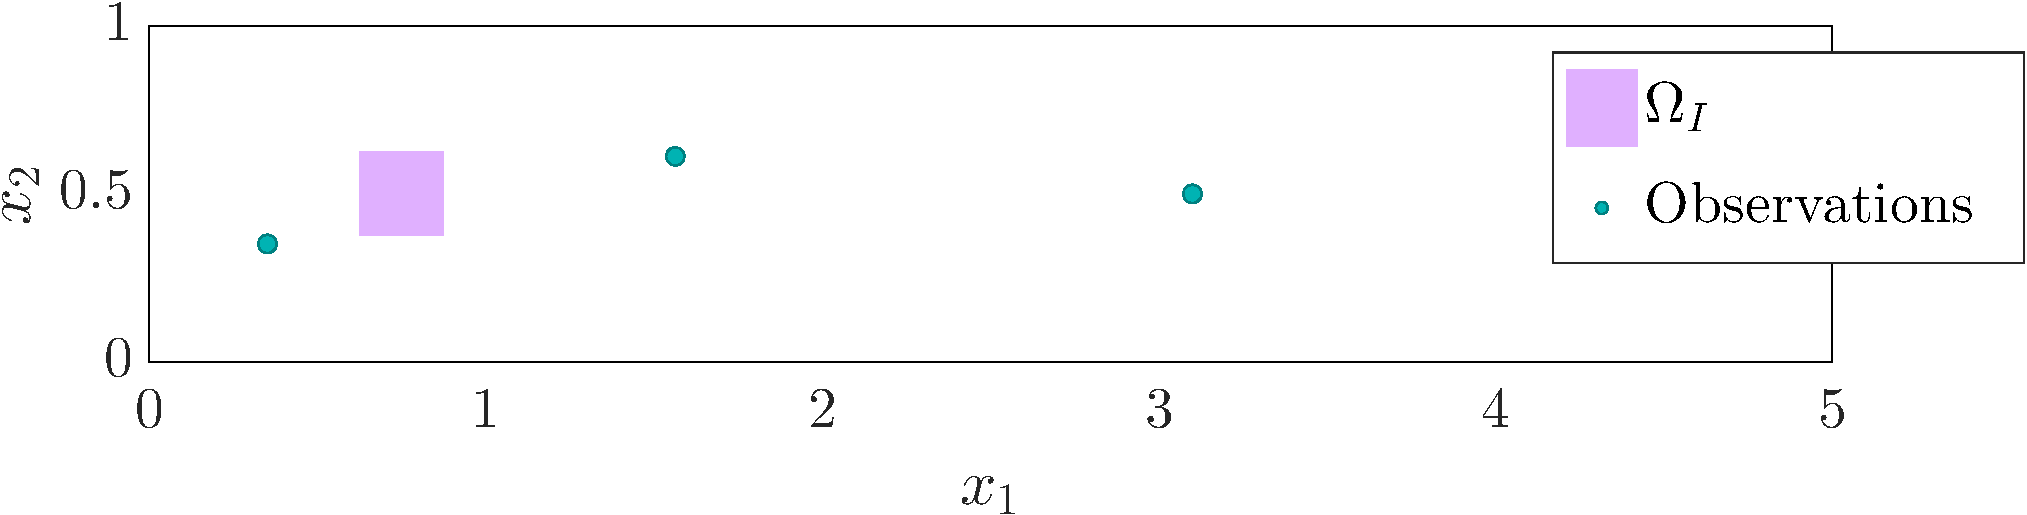
\includegraphics[width=0.8\textwidth]{baseSeries/setup_3_3.pdf}
\caption{Locations of the observations and the QoI region.}
\label{fig:baseSetup}
\end{figure}
%

For the numerical simulations, we use the finite element method (FEM), employing a continuous Galerkin formulation with Lagrange elements. We use the \texttt{libMesh} library~\cite{libMeshPaper} for the FEM calculations. The domain is discretized by a regular mesh of quadrilaterals, with 250 and 50 elements along the $x_1$ and $x_2$ directions, respectively, for a total of 12,500 elements, resulting in 12,801 degrees of freedom per variable. The diffusion coefficient is such that the cell P\'{e}clet number never exceeds 0.1, and thus no stabilization is required.

Synthetic observations consisting of the state at three points in the domain are artificially generated by running the high-fidelity model on a finer mesh with the true forcing field
%
\begin{equation}
f_{true}(x_1,x_2)=
\begin{cases}
1.0 & \textrm{if }(x_1,x_2)\in[0.125,0.375]\times[0.125,0.375] \\
0.8 & \textrm{if }(x_1,x_2)\in[2.375,2.625]\times[0.375,0.625] \\
0 & \textrm{otherwise}.
\end{cases}
\end{equation}
%
%
%------------------------------------------------------------%
\subsubsection{Adaptive Model Refinement Results} \label{sec:cdvcdrBaseRef}
%------------------------------------------------------------%
%

We now present the results for solving the inference problem using \Cref{alg:refSeries}. Once the QoI error estimate is calculated using \Cref{eq:finErrExp}, the error estimate is then decomposed into local contributions. At each iteration, based on this decomposition, we choose the basis functions with the largest error contributions until an additional 5\% of the elements has been marked for refinement. This is repeated until the estimated absolute relative error in the QoI, calculated as $\epsilon_i/(\epsilon_i+I(q_{MF_i},u_{MF_i}))$, is less than $1\%$.

\Cref{fig:baseRef} shows the local error contributions, as well as the subdomains where the low- and high-fidelity models are used, for the series of mixed-fidelity models thus generated. 
%
\begin{figure}[htbp]
%\captionsetup[subfloat]{captionskip=-5pt}
\centering
\subfloat[LF $\equiv$ MF$_0$ ($0\%$ HF)]{
  \includegraphics[width=0.46\textwidth]{baseSeries/cd_cdr_LF_divvy.jpeg}
  \includegraphics[width=0.49\textwidth]{baseSeries/err_breakdown_LF.jpeg}
  \label{fig:baseRef0}
} \\
\subfloat[MF$_1$ ($5\%$ HF)]{
  \includegraphics[width=0.46\textwidth]{baseSeries/cd_cdr_MF01_divvy.jpeg}
  \includegraphics[width=0.49\textwidth]{baseSeries/err_breakdown_MF01.jpeg}
} \\
\subfloat[MF$_2$ ($10\%$ HF)]{
  \includegraphics[width=0.46\textwidth]{baseSeries/cd_cdr_MF02_divvy.jpeg}
  \includegraphics[width=0.49\textwidth]{baseSeries/err_breakdown_MF02.jpeg}
} \\
\caption{Left: Multi-fidelity refinement over the domain (low-fidelity convection-diffusion model used in red portion, high-fidelity convection-diffusion-reaction model used in blue portion). Right: local error contributions. }
\label{fig:baseRef}
\end{figure}
%
Note that the error contribution of each basis function whose support is entirely within the high-fidelity regions is zero.

We see that the largest local error contributions are concentrated in the QoI region and around the observation location closest to the QoI. In the first decomposition of the error (\Cref{fig:baseRef0}), the region where the elemental error is greatest is around the leftmost observation location. Since the constraining model is an elliptic PDE, with weak convection, information flow is localized, and is weakly convected from left to right. Therefore, for the calculation of the QoI, it is most important to refine the region near the leftmost observation location, and then around the QoI region. After that, the error decomposition suggests refinement in regions upstream and around the middle observation location, and then the rightmost observation location.

\Cref{fig:baseErr} shows the true and estimated absolute relative errors in the QoI for the various mixed-fidelity models generated by \Cref{alg:refSeries}; the true and estimated relative errors are calculated relative to the true and estimated high-fidelity QoI, respectively. In this case, we see that QoI error of $1\%$ is attained with a mixed-fidelity model where the high-fidelity model is used in only about $10\%$ of the domain. We note that while here the error is seen to decrease with increasing refinement, in general there is no guarantee that either the error in the QoI or the relative error in the error estimate will decrease monotonically as more of the domain is refined.
%
\begin{figure}[htbp]
\centering
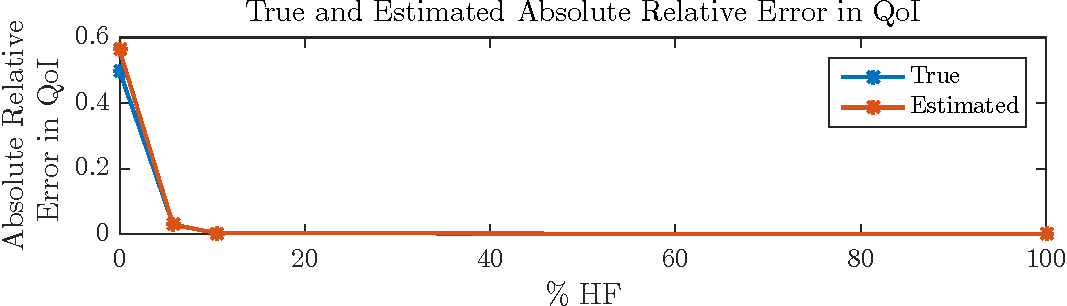
\includegraphics[width=0.8\textwidth]{baseSeries/err_est.pdf}
\caption{True and estimated absolute relative error in QoI, plotted as a function of the percentage area of the domain in which the high-fidelity convection-diffusion-reaction model is used.}
\label{fig:baseErr}
\end{figure}
%

%------------------------------------------------------------%
\subsubsection{Interaction of Observations and QoI} \label{sec:qoivdata}
%------------------------------------------------------------%
%
The error estimate decomposition suggests the use of the high-fidelity model in areas of the domain that are important to the interaction between the observations and QoI; the interaction between these two can be complex, and the areas suggested for refinement may be nonintuitive. To see this, we compare the error estimate decomposition for three sizes of the QoI region $\Omega_I$ given the same set of observation locations, and for three nested sets of observation locations given the same QoI region. For the sake of illustration, we make two refinement iterations for each combination of observations and QoI region, regardless of the magnitude of the relative error estimate. However, in conducting the numerical experiments, it was observed that the number of iterations needed to achieve a given tolerance tended to increase as the QoI region increased.

\Cref{fig:qoiStudy} shows the domain for three cases considered, with the same set of observations but increasingly large, nested QoI regions $\Omega_I$.
The error decompositions for each case are also shown in \Cref{fig:qoiStudy}. The bottom row gives the baseline case presented in \Cref{sec:cdvcdrBaseRef}, although here we choose the basis functions $i$ whose error $\varepsilon_i$ are among the largest $5\%$, rather than only enough basis functions to cover 5\% of the domain in their support, so the proportion of elements marked for refinement in each iteration will be slightly larger than in \Cref{sec:cdvcdrBaseRef}. Although refinement is still most important around the observation location closest to $x_1=0$, as the QoI region expands the other two observation locations become more important in that the error decomposition suggests refinement around them earlier. As the QoI region expands, it is also more clearly noticeable that refinement is not equally important in all parts of the QoI region.

\begin{figure}[htbp]
\centering
\captionsetup{justification=centering}
\subfloat[Locations of observations and QoI region $\Omega_I$][Locations of \\observations and \\QoI region $\Omega_I$]{
  %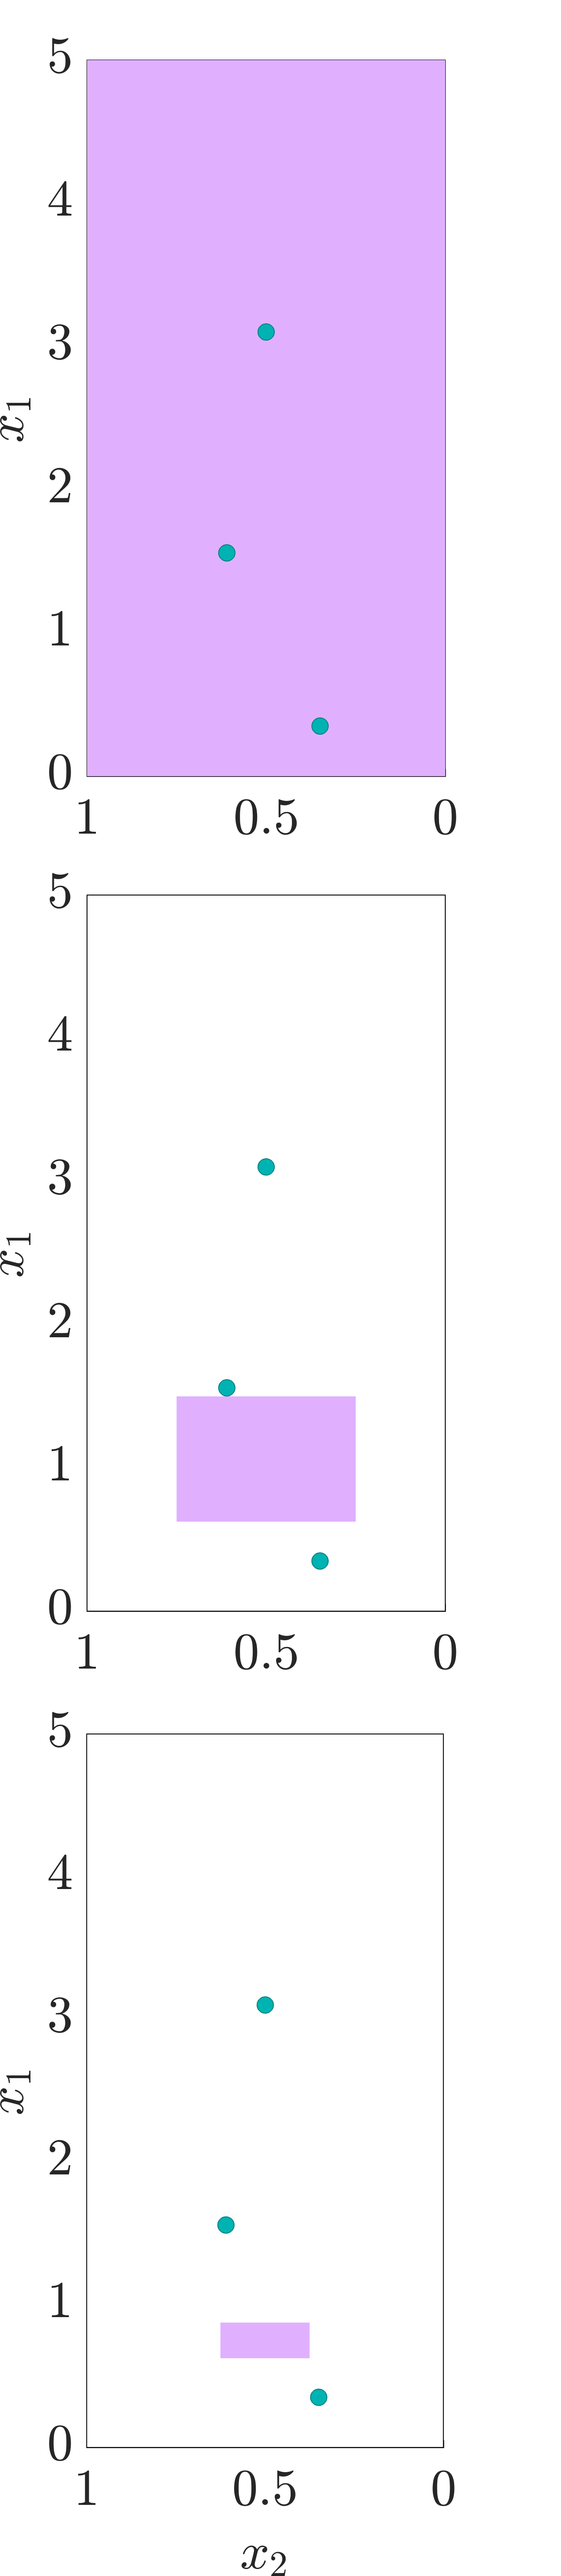
\includegraphics[width=0.23\textwidth]{vs_qoi/vs_qoi_setup.png}
  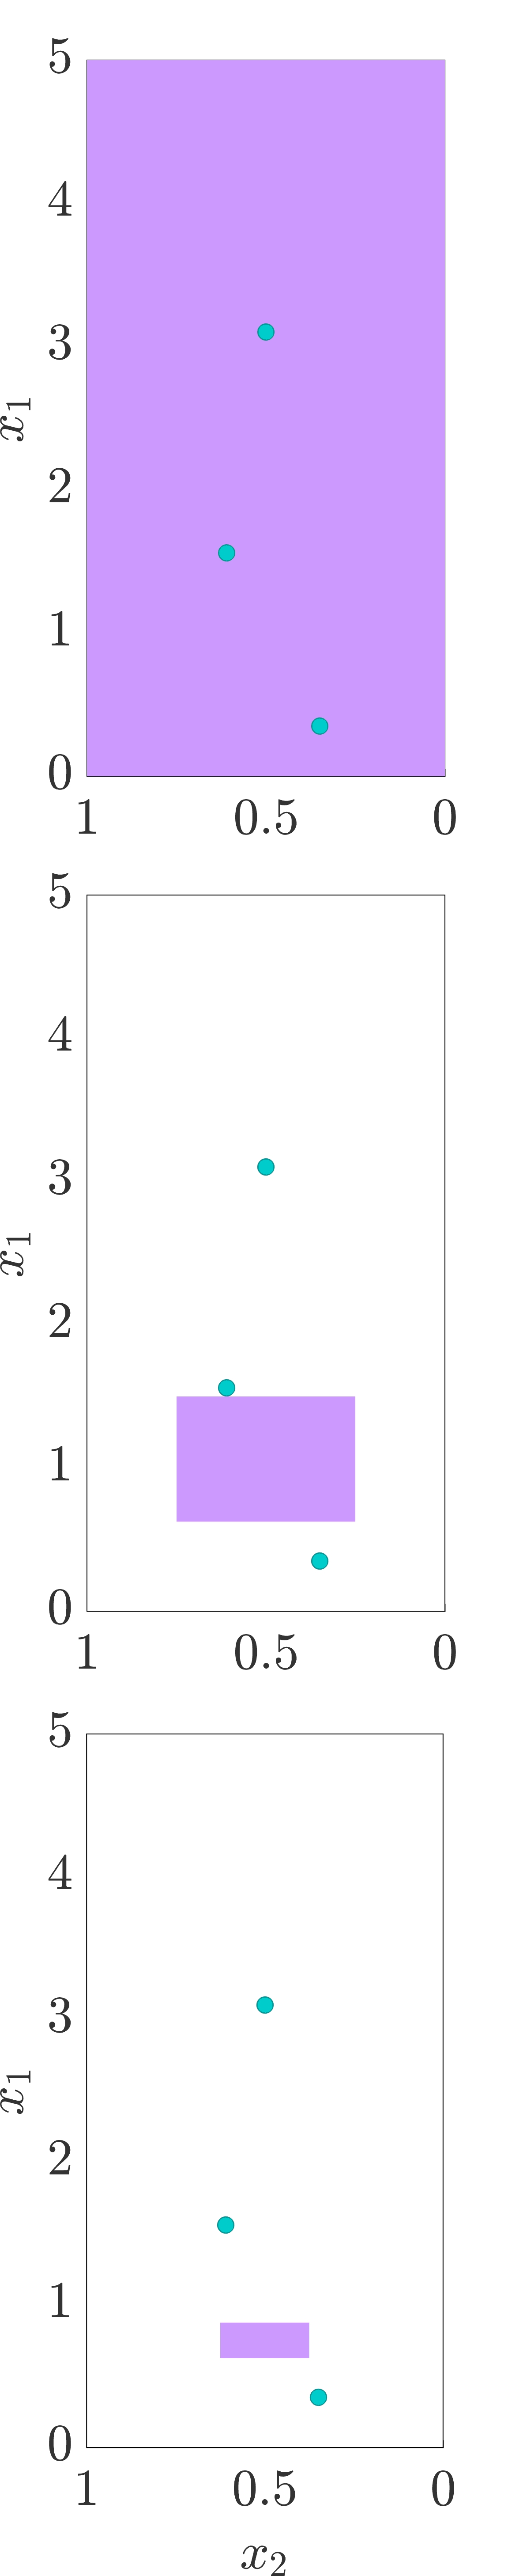
\includegraphics[width=0.21\textwidth]{vs_qoi/vs_qoi_setup_sidetrim.jpeg}
  \label{subfig:obsSetup}
}
\captionsetup{justification=centering}
\subfloat[MF$_0$ ($0\%$ HF)][MF$_0$ \\($0\%$ HF)]{
  %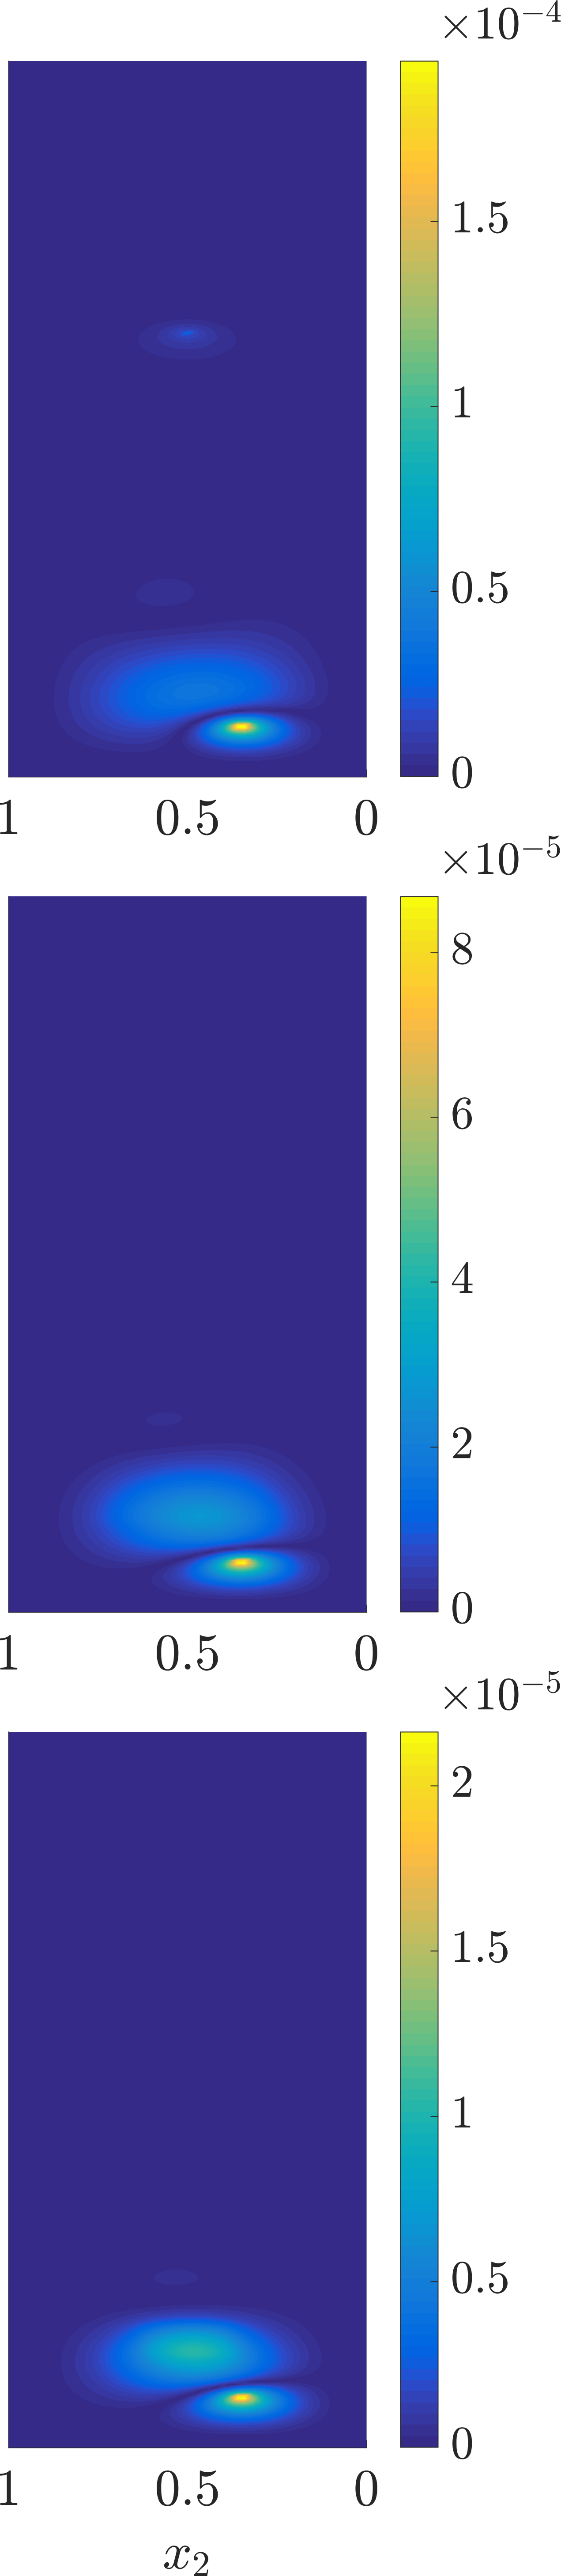
\includegraphics[width=0.23\textwidth]{vs_qoi/vs_qoi_err0.png}
  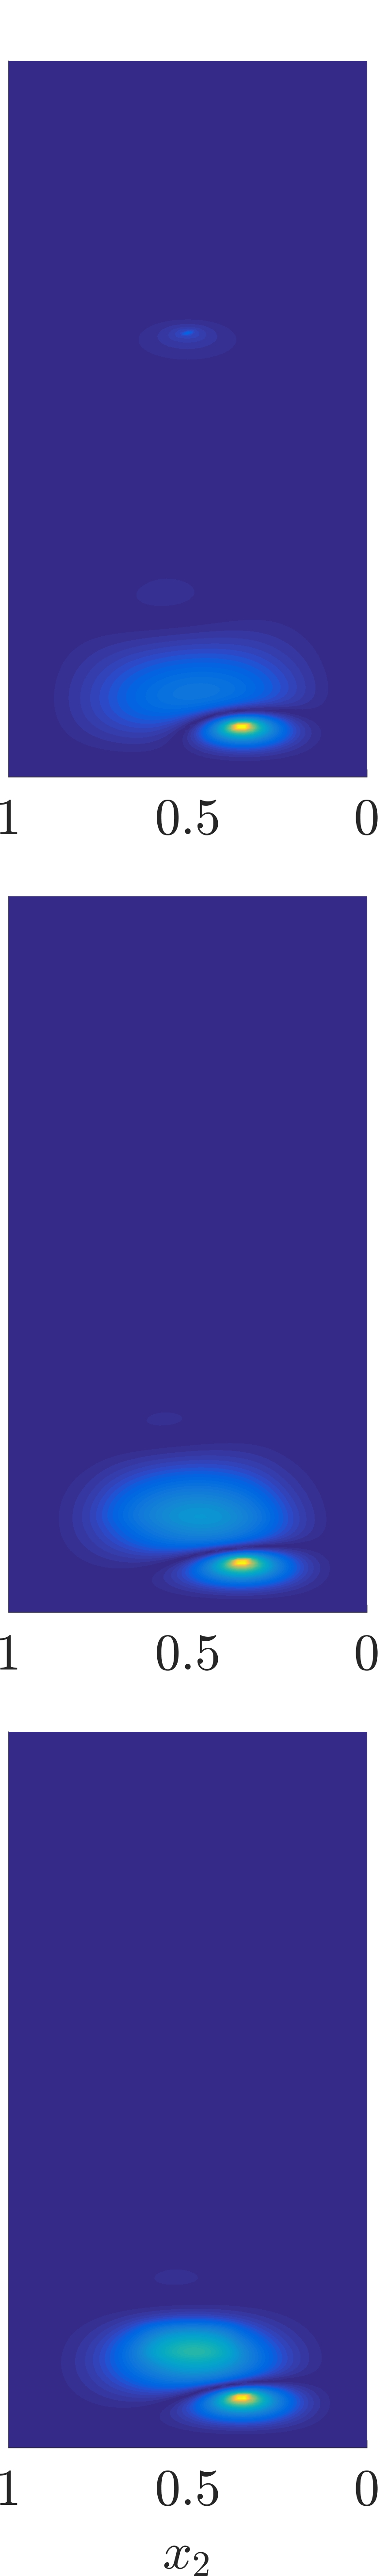
\includegraphics[width=0.16\textwidth]{vs_qoi/vs_qoi_err0_nobar.jpeg}
  \label{subfig:obsLF}
}
\captionsetup{justification=centering}
\subfloat[MF$_1$ ($\sim5\%$ HF)][MF$_1$ \\($\sim5\%$ HF)]{
  %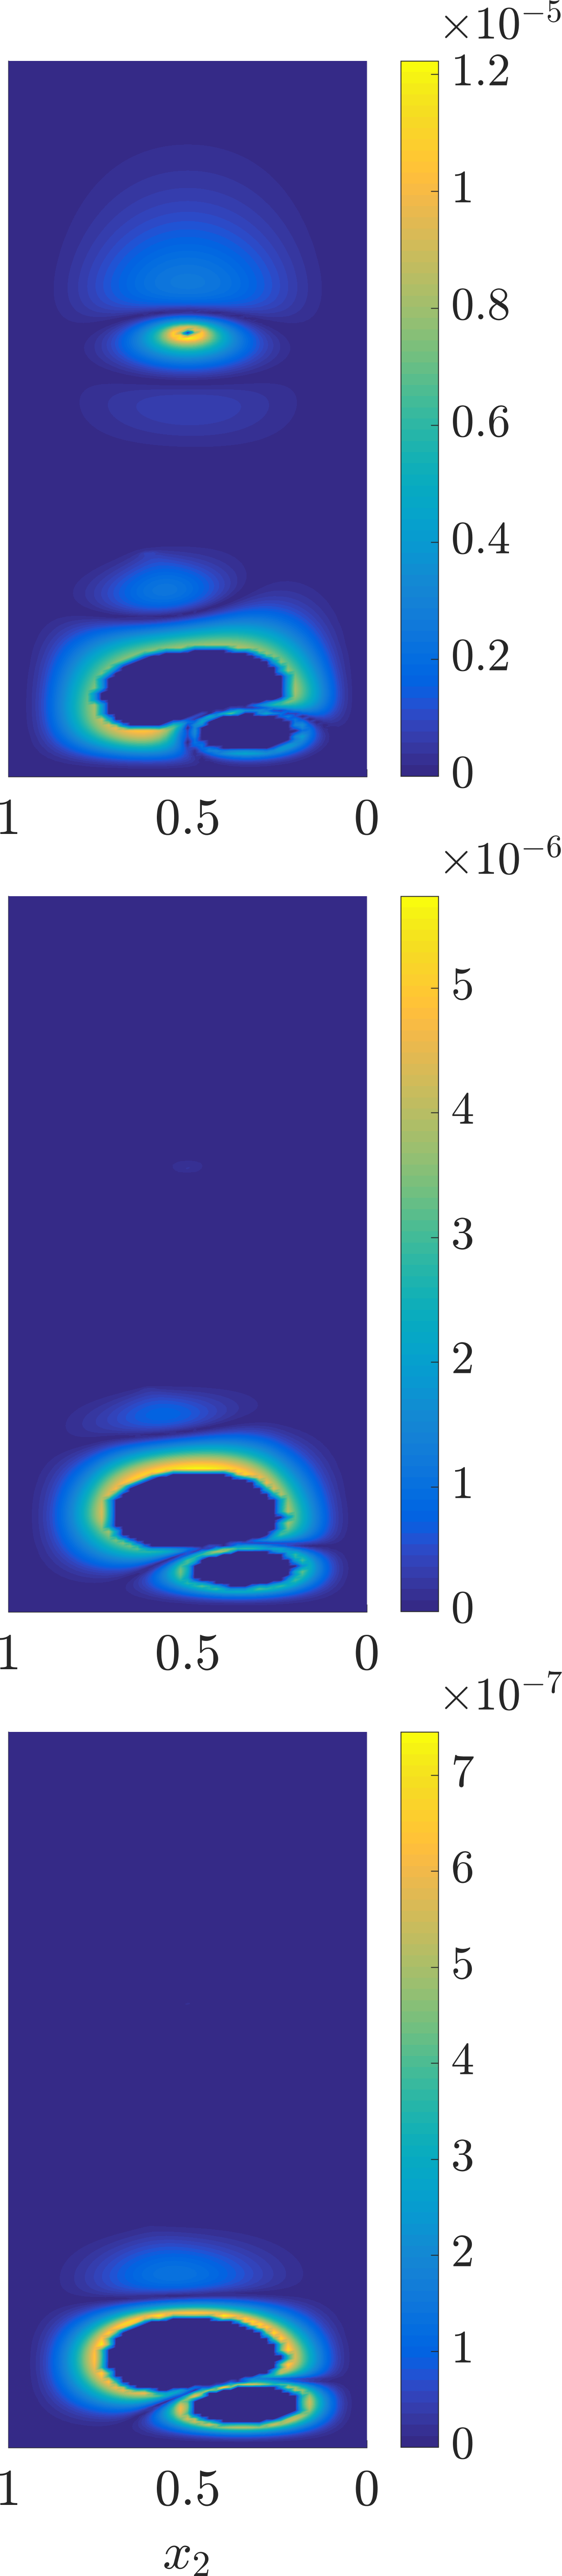
\includegraphics[width=0.23\textwidth]{vs_qoi/vs_qoi_err1.png}
  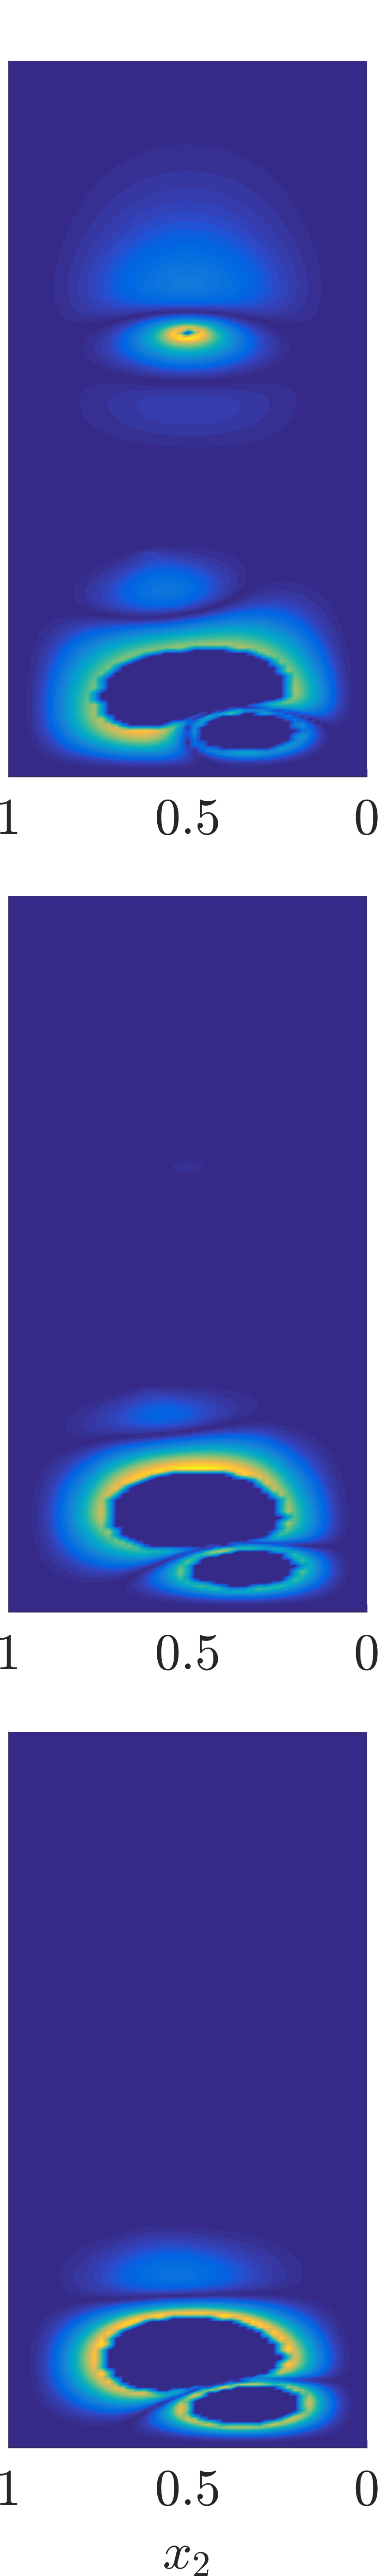
\includegraphics[width=0.16\textwidth]{vs_qoi/vs_qoi_err1_nobar.jpeg}
}
\captionsetup{justification=centering}
\subfloat[MF$_2$ ($\sim10\%$ HF)][MF$_2$ \\($\sim10\%$ HF)]{
  %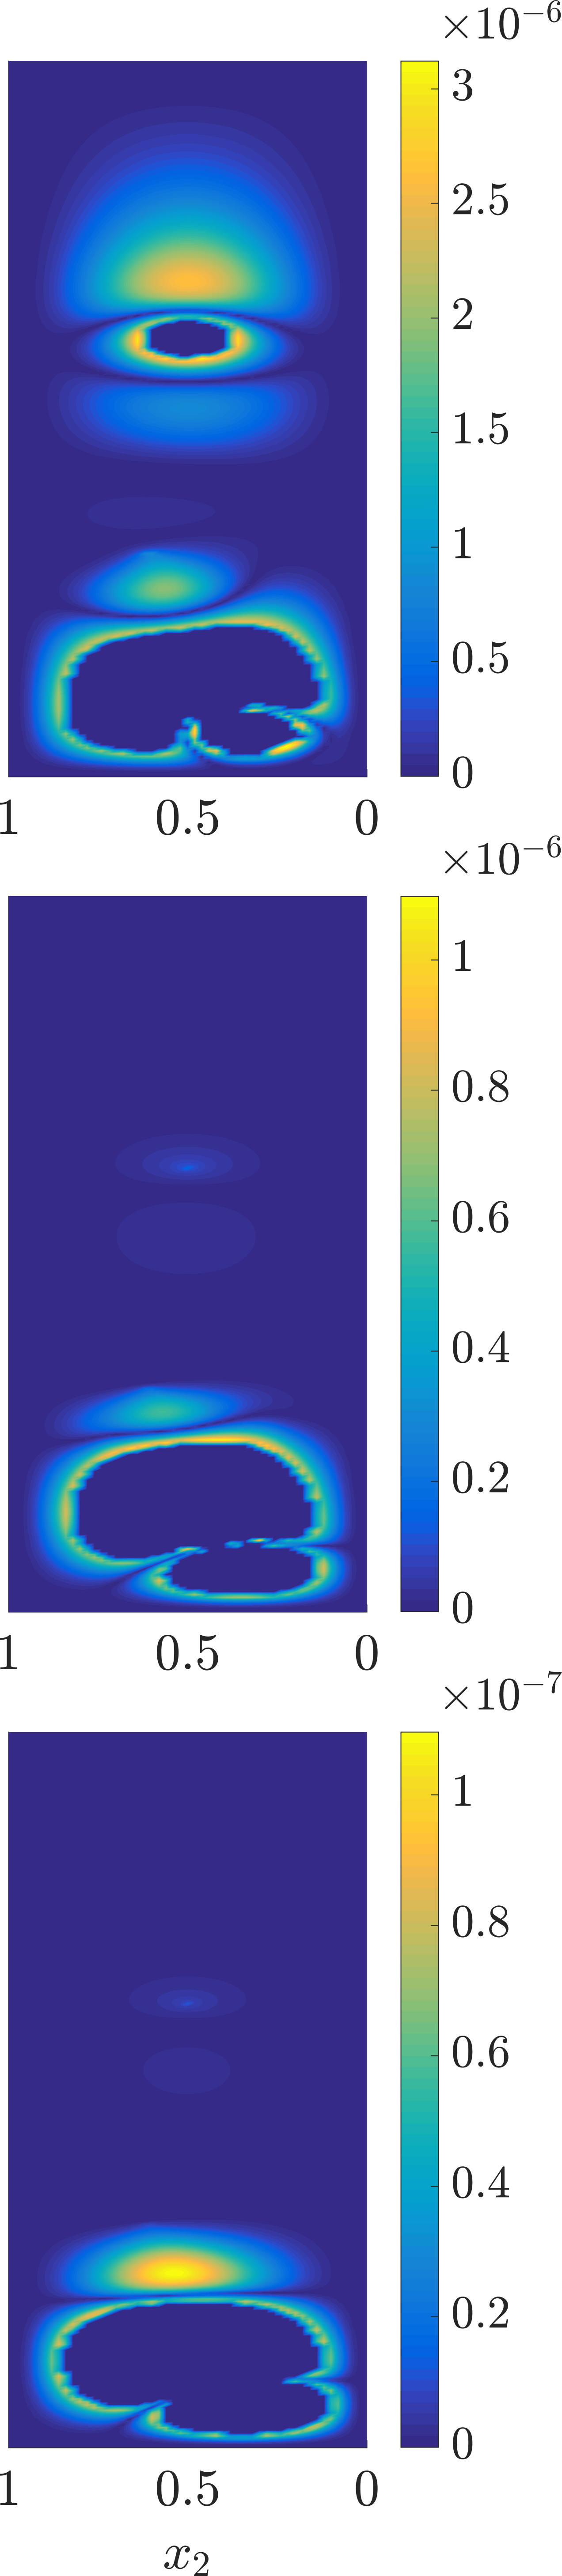
\includegraphics[width=0.23\textwidth]{vs_qoi/vs_qoi_err2.png}
  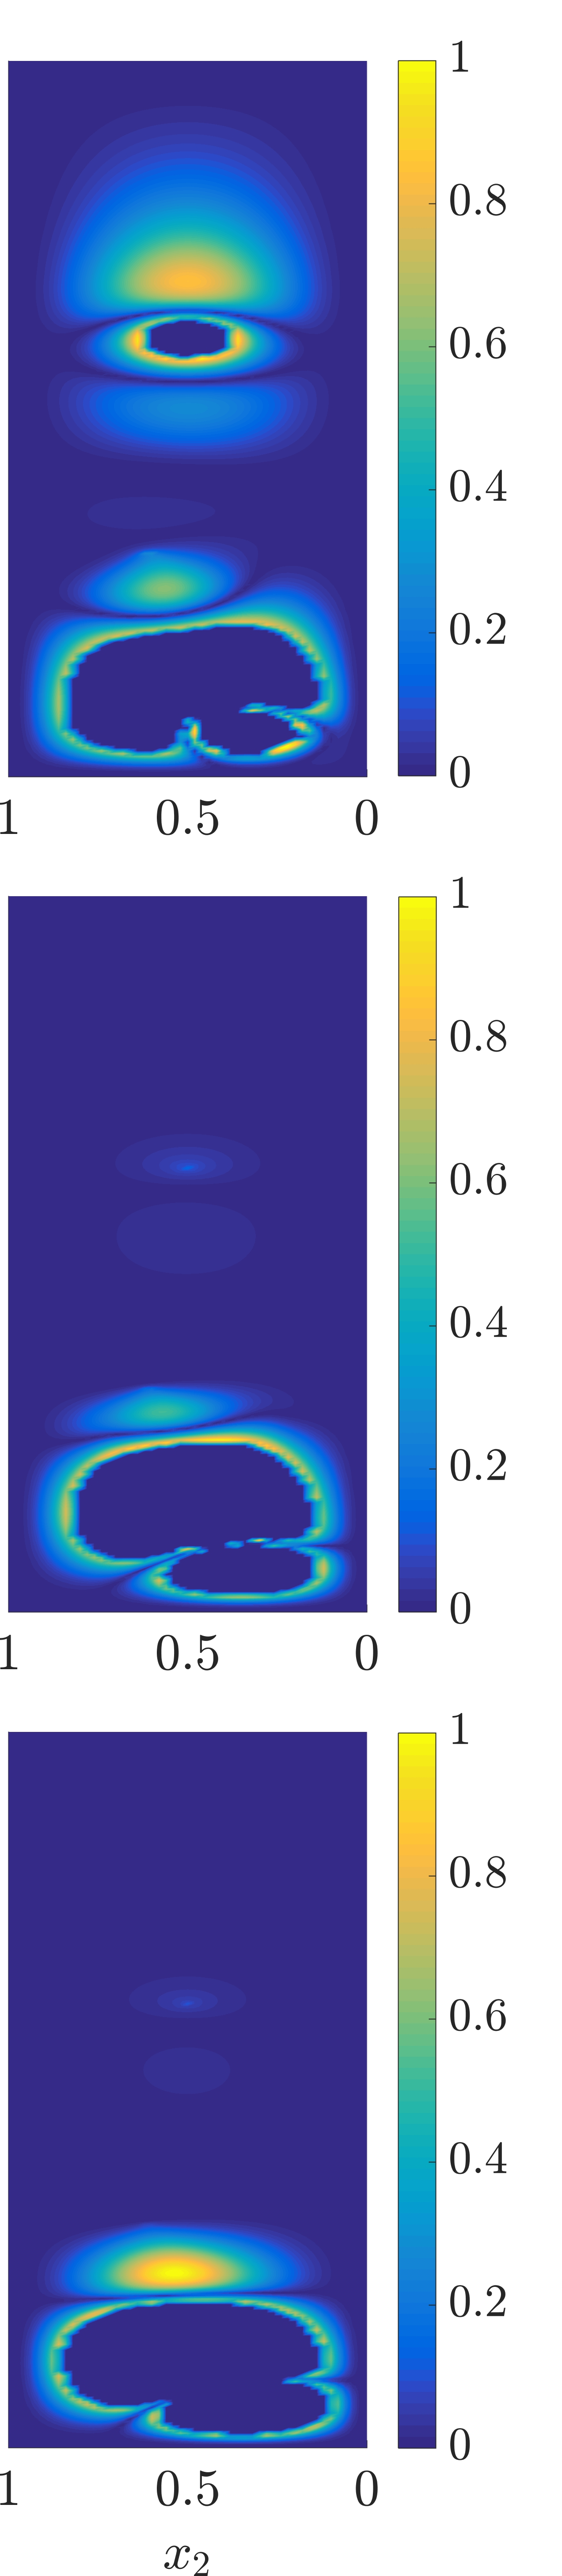
\includegraphics[width=0.23\textwidth]{vs_qoi/vs_qoi_err2_barnorm.jpeg}
  \label{subfig:obsMFlast}
}
  \caption{Effects of increasing the QoI region. Column \protect\subref{subfig:obsSetup}: configuration of observations (teal points) and QoI region (purple box). Columns \protect\subref{subfig:obsLF}--\protect\subref{subfig:obsMFlast}: the relative error estimate decompositions for different mixed-fidelity models, relative to the largest localized error contribution; note the locations of regions of relatively large error compared to the observation locations and QoI region.}
  \label{fig:qoiStudy}
\end{figure}

\Cref{fig:dataStudy} shows another set of cases considered, now with the same QoI region $\Omega_I$ but with increasing, nested sets of observations.
The error decomposition for the three cases is shown in \Cref{fig:dataStudy}. The bottom row is the same as that in \Cref{fig:qoiStudy}. Refinement appears to be consistently most important around the observation location closest to $x_1=0$ and the QoI region. However, as more observation locations are added, it becomes no longer necessarily true that refinement becomes less important around observation locations as their distance from the QoI region increases. In the second and third rows, one can see that after the areas around the QoI region and the two closest observation locations have been refined, the next area to be refined is not around the third closest observation location, but rather around one near the middle of the domain. This suggests that interactions between observation locations and the QoI may be non-intuitive, and in these cases a rigorous method for forming a mixed-fidelity model leads to well-supported modeling choices.

\begin{figure}[htbp]
\centering
\captionsetup{justification=centering}
\subfloat[Locations of observations and QoI region $\Omega_I$][Locations of \\observations and \\QoI region $\Omega_I$]{
  %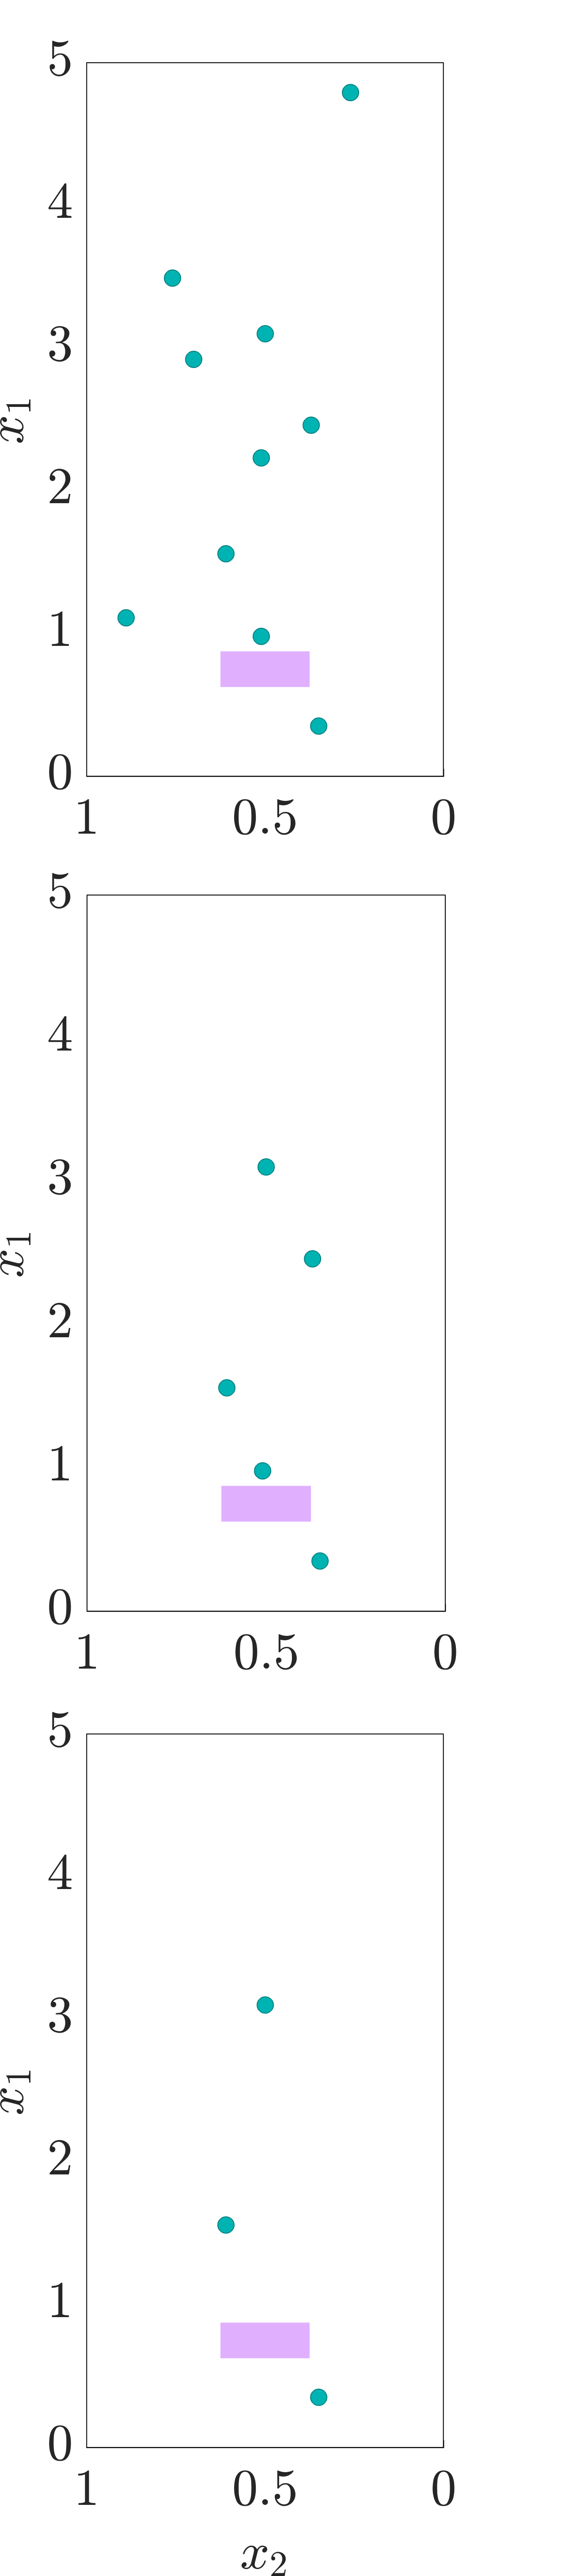
\includegraphics[width=0.23\textwidth]{vs_data/vs_data_setup.png}
  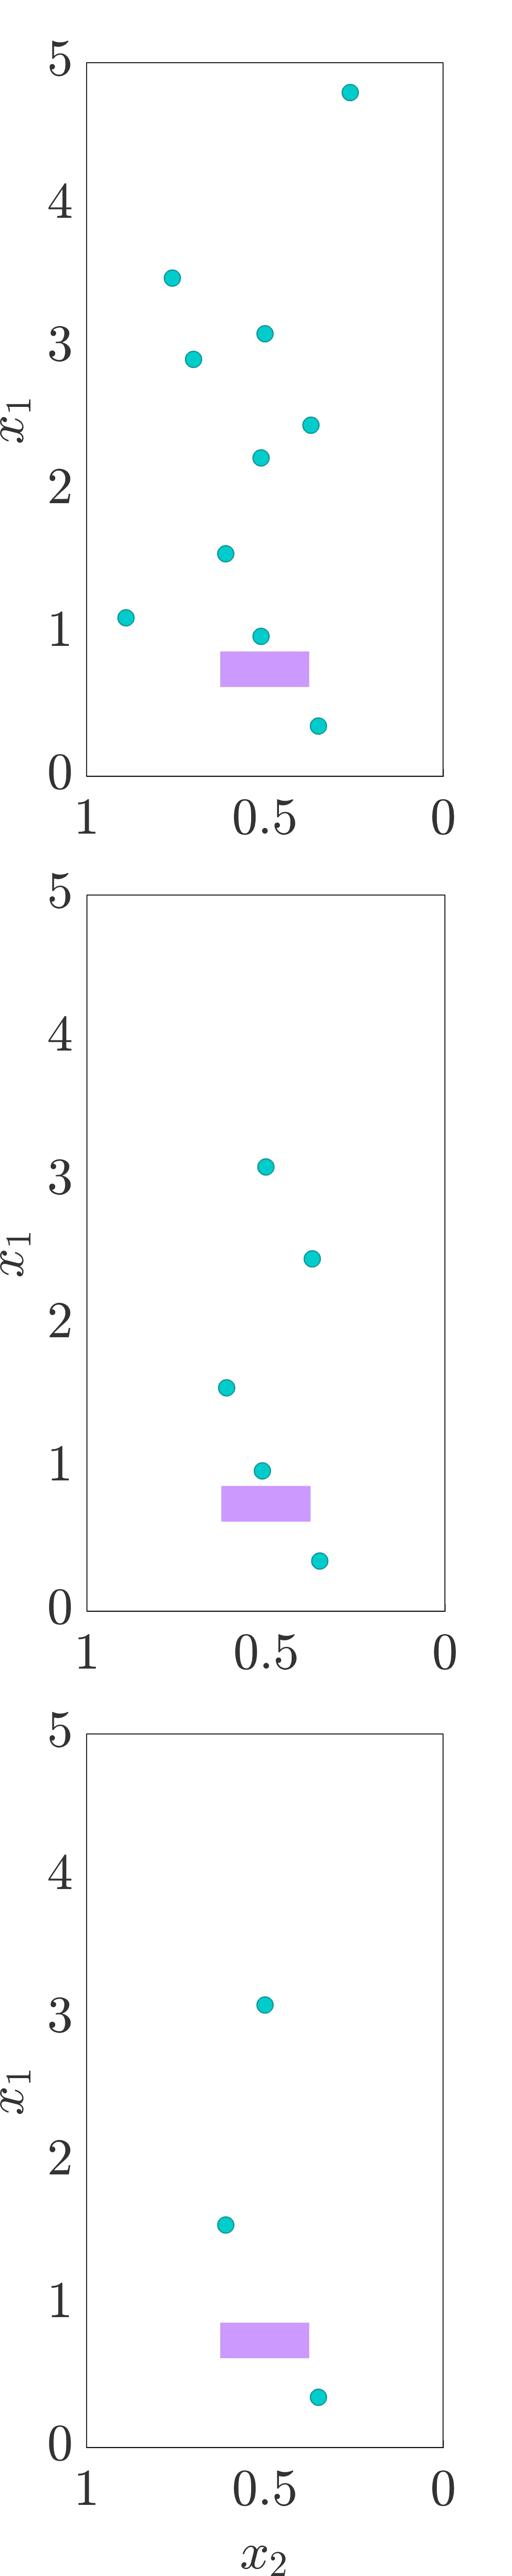
\includegraphics[width=0.21\textwidth]{vs_data/vs_data_setup_sidetrim.jpeg}
  \label{subfig:obsSetup2}
}
\captionsetup{justification=centering}
\subfloat[MF$_0$ ($0\%$ HF)][MF$_0$ \\($0\%$ HF)]{
  %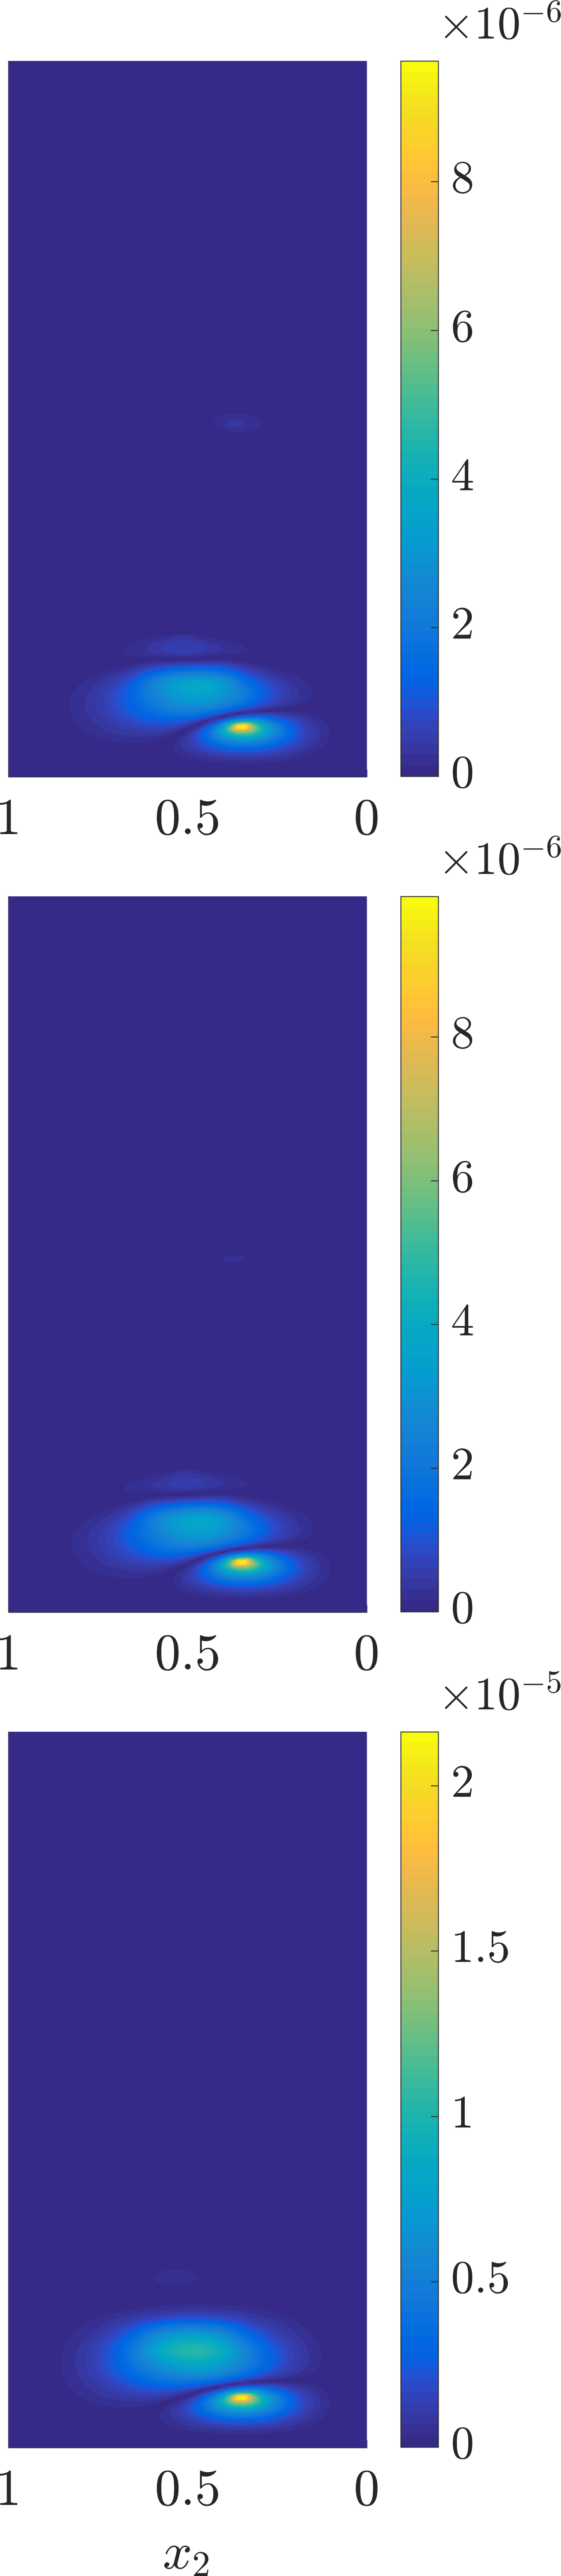
\includegraphics[width=0.23\textwidth]{vs_data/vs_data_err0.png}
  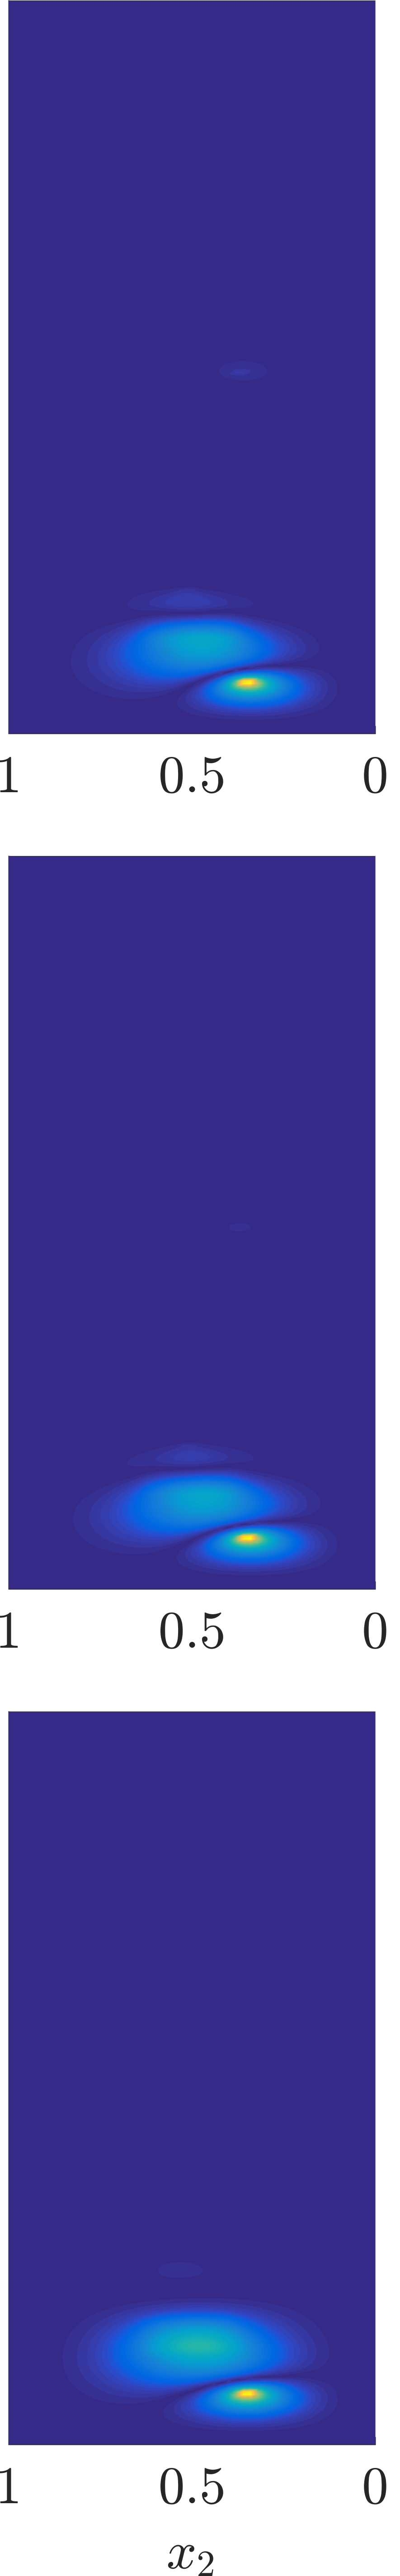
\includegraphics[width=0.16\textwidth]{vs_data/vs_data_err0_nobar.jpeg}
  \label{subfig:obsLF2}
}
\captionsetup{justification=centering}
\subfloat[MF$_1$ ($\sim5\%$ HF)][MF$_1$ \\($\sim5\%$ HF)]{
  %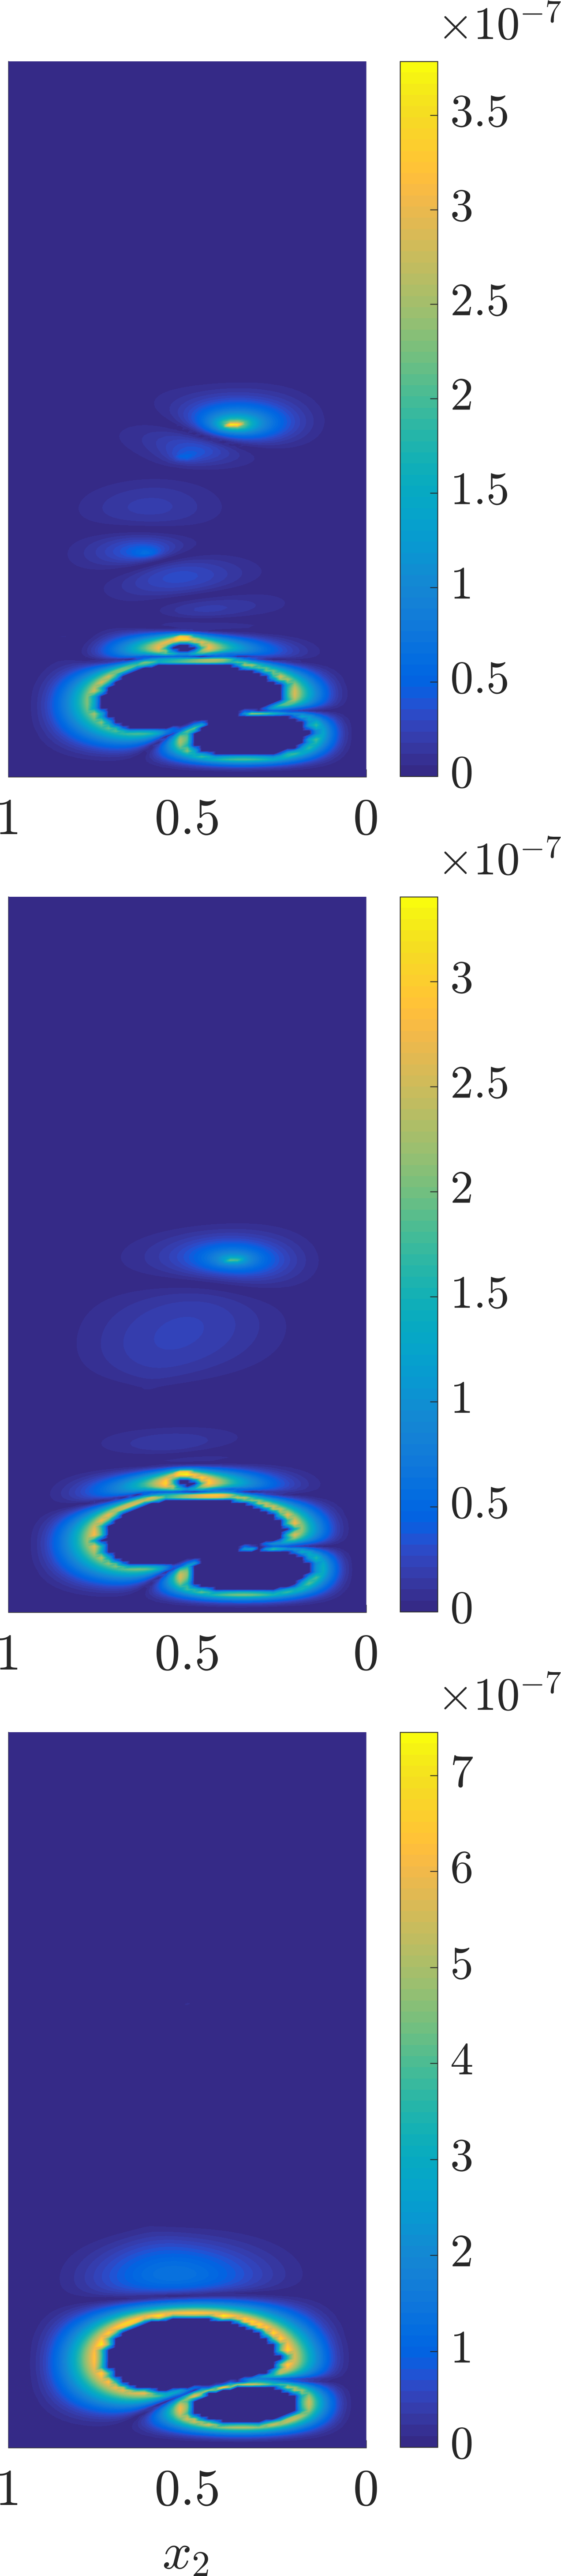
\includegraphics[width=0.23\textwidth]{vs_data/vs_data_err1.png}
  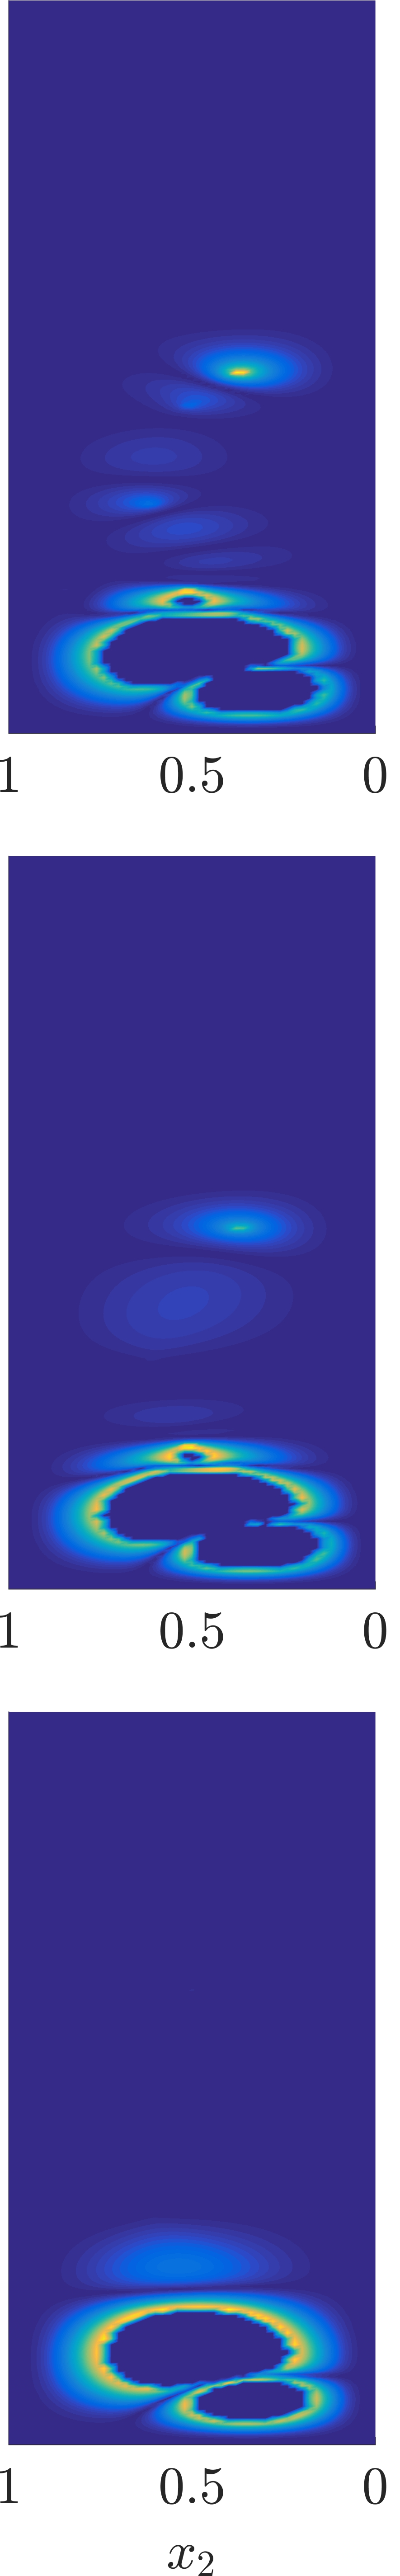
\includegraphics[width=0.16\textwidth]{vs_data/vs_data_err1_nobar.jpeg}
}
\captionsetup{justification=centering}
\subfloat[MF$_2$ ($\sim10\%$ HF)][MF$_2$ \\($\sim10\%$ HF)]{
  %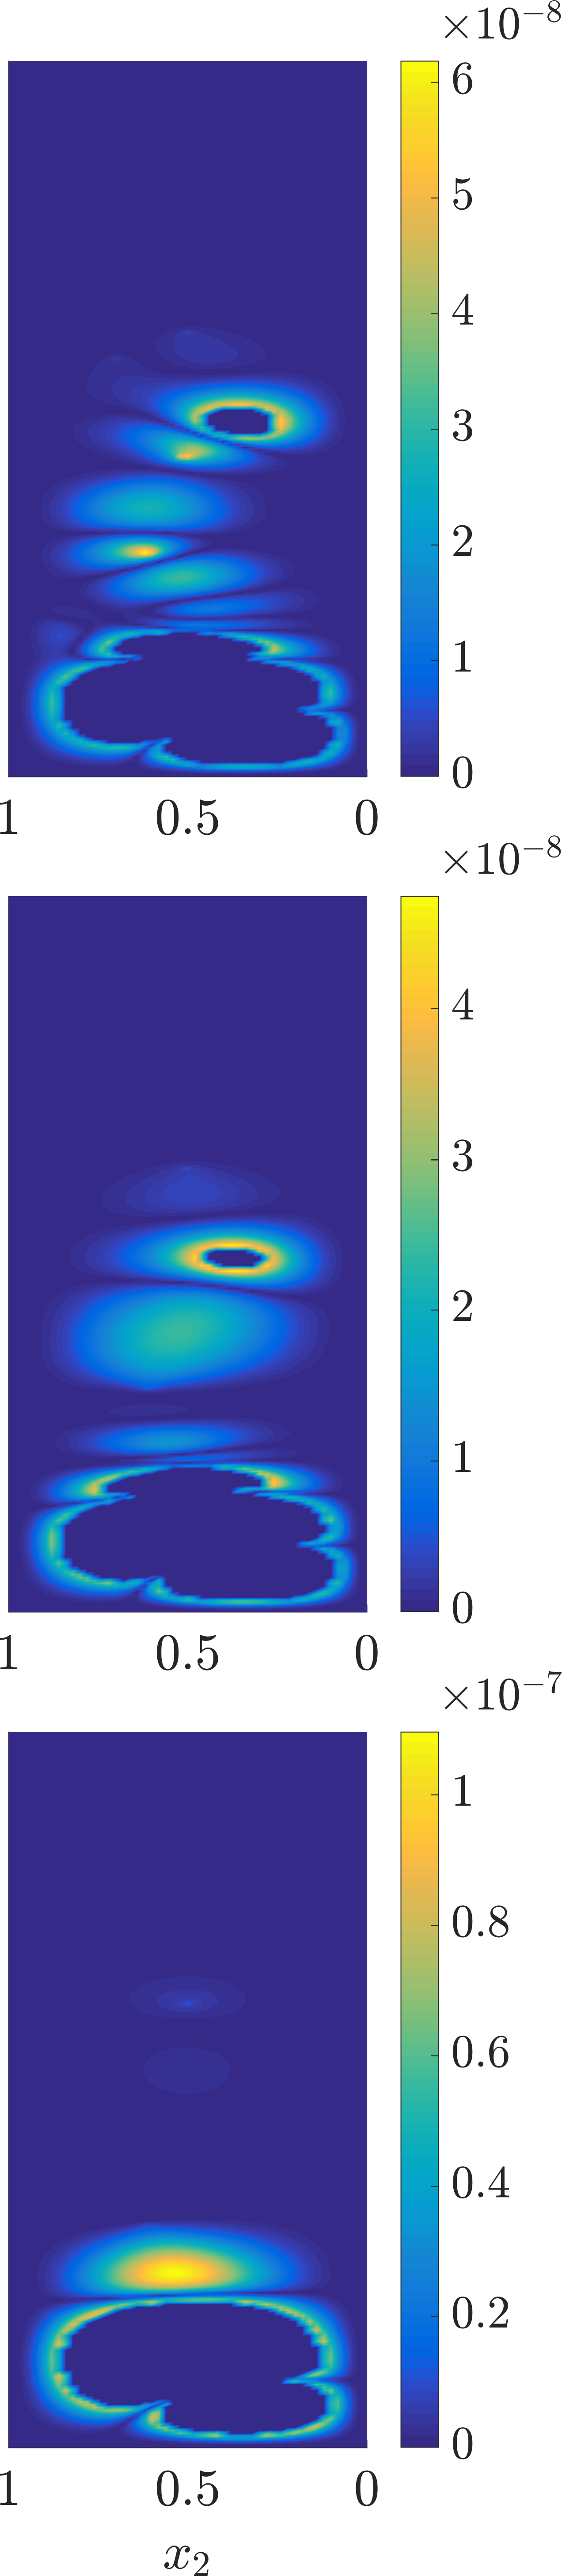
\includegraphics[width=0.23\textwidth]{vs_data/vs_data_err2.png}
  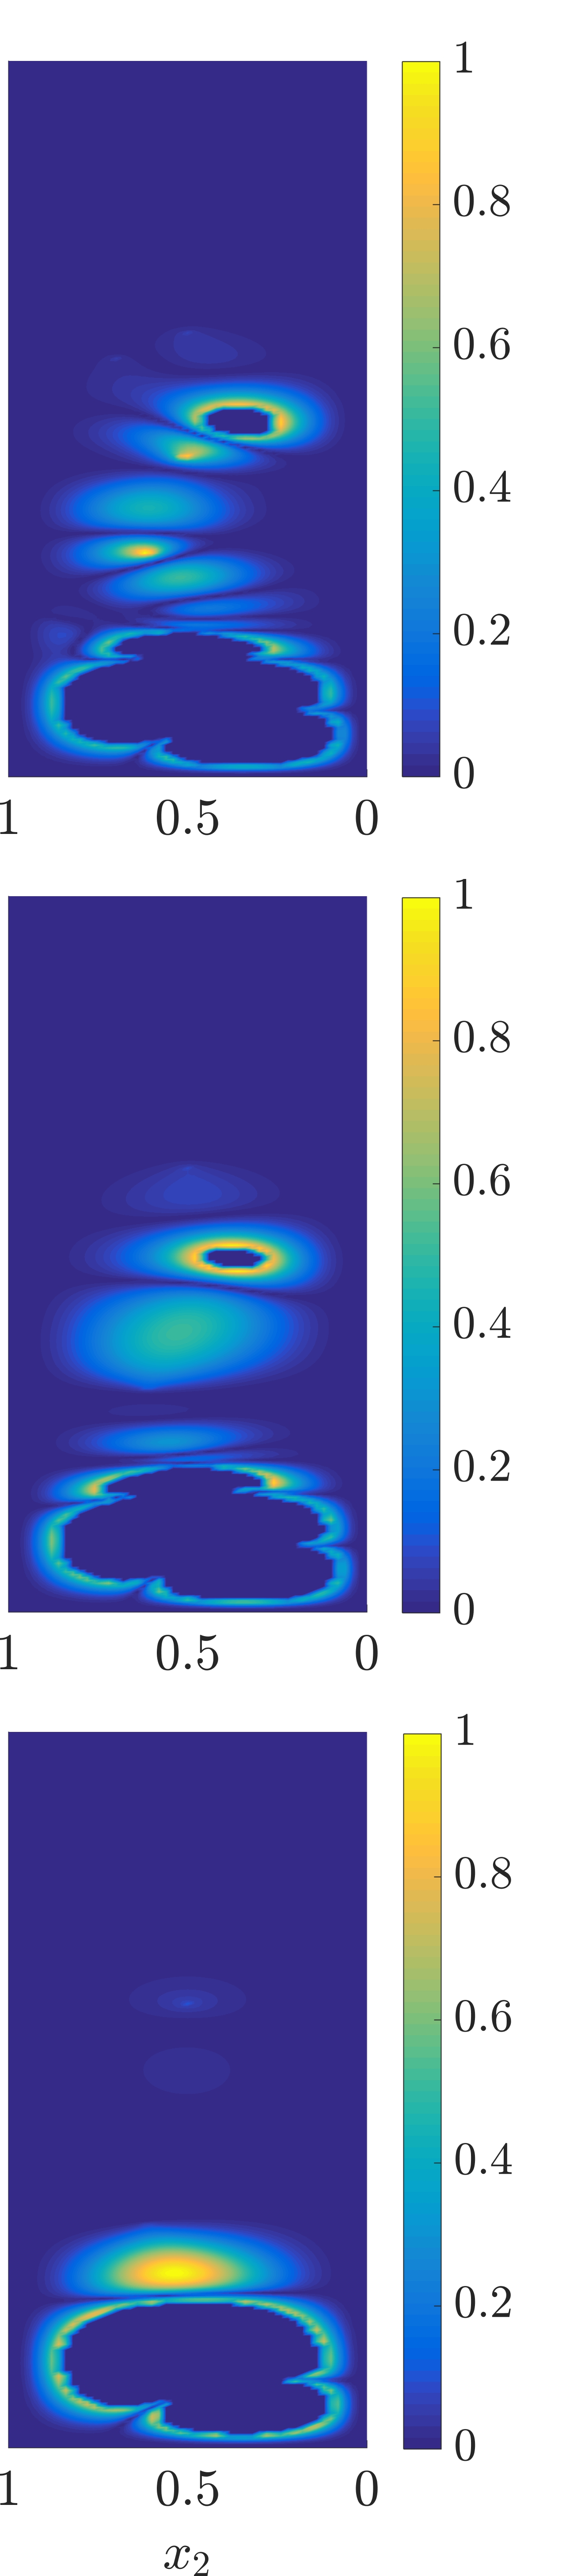
\includegraphics[width=0.23\textwidth]{vs_data/vs_data_err2_barnorm.jpeg}
  \label{subfig:obsMFlast2}
}
  \caption{Effects of increasing the number of observations. Column \protect\subref{subfig:obsSetup2}: configuration of observations (teal points) and QoI region (purple box). Columns \protect\subref{subfig:obsLF2}--\protect\subref{subfig:obsMFlast2}: the relative error estimate decompositions for different mixed-fidelity models, relative to the largest localized error contribution; note the locations of regions of relatively large error compared to the observation locations and QoI region.}
  \label{fig:dataStudy}
\end{figure}

%------------------------------------------------------------------------------------------------------------------------%
\subsection{Variable Parameterization: Constant vs.\ Field Parameters} \label{sec:constvfield}
%------------------------------------------------------------------------------------------------------------------------%

In this subsection, we consider two models which differ in the space to which the parameter belongs, with the low-fidelity model having fewer degrees of freedom. 

%------------------------------------------------------------%
\subsubsection{Problem Setup}
%------------------------------------------------------------%

We consider the same high-fidelity model as in \Cref{sec:cdvcdr}:
\begin{equation}
k_d\nabla^2 u - \vec{V}\cdot\nabla u + k_ru^2= f(q),\quad q\in U,
\end{equation}
with the same diffusion coefficient $k_d = 0.1$  and reaction coefficient $k_r = -42$. The low-fidelity model
\begin{equation}
k_d\nabla^2 u - \vec{V}\cdot\nabla u + k_ru^2= f(q),\quad q\in\R
\end{equation}
differs from the high-fidelity model only in that the parameter $q$ is a constant instead of a field. The intermediate mixed-fidelity models thus have parameter fields that are constant over the subregions of the domain where the low-fidelity model is used. For ease of implementation, we require that the resulting parameter field remain continuous at the interface between the low-fidelity and high-fidelity subdomains, although this constraint is not necessary for the theory to hold. The domain, mesh, boundary conditions, and velocity field, as well as the observations, unknown parameters to be inferred, and QoI, remain the same as described in \Cref{sec:cdvcdr}. As the inverse problem is ill-posed, except when the low-fidelity model is used throughout the domain, regularization is used; the Tikhonov regularization term in \Cref{eq:invOpt_obj} is $R(q)=\frac{\beta}{2}\int_\Omega \|\nabla f(q)\|_2^2+f(q)^2\:\textrm{d}A$, where $\beta=10^{-3}$ is a regularization coefficient. 

%------------------------------------------------------------%
\subsubsection{Adaptive Model Refinement Results}
%------------------------------------------------------------%

As with the previous examples in \Cref{sec:cdvcdr}, the decomposition of the error estimate is used to select additional regions of the domain in which to use the high-fidelity model. The number of degrees of freedom in the inverse problem increases with the proportion of the domain in which the high-fidelity model is used. With each iteration, an additional $10\%$ of the elements are marked for refinement. This is repeated until the estimated absolute relative error in the QoI is less than $1\%$.

\Cref{fig:svfRef} shows the local error contributions, as well as the subdomains where the low- and high-fidelity models are used, for the first two and last mixed-fidelity model thus generated. 
%
\begin{figure}[htbp]
\centering
\subfloat[MF$_0$ ($0\%$ HF)]{
	\includegraphics[width=0.46\textwidth]{svf/cd_cdr_LF_divvy.jpeg}
  \includegraphics[width=0.49\textwidth]{svf/err_breakdown_LF.jpeg}
} \\
\subfloat[MF$_1$ ($10\%$ HF)]{
	\includegraphics[width=0.46\textwidth]{svf/cd_cdr_MF01_divvy.jpeg}
  \includegraphics[width=0.49\textwidth]{svf/err_breakdown_MF01.jpeg}
} \\
\subfloat[MF$_2$ ($20\%$ HF)]{
  \includegraphics[width=0.46\textwidth]{svf/cd_cdr_MF02_divvy.jpeg}
  \includegraphics[width=0.49\textwidth]{svf/err_breakdown_MF02.jpeg}
} \\
\subfloat[MF$_6$ ($60\%$ HF)]{
	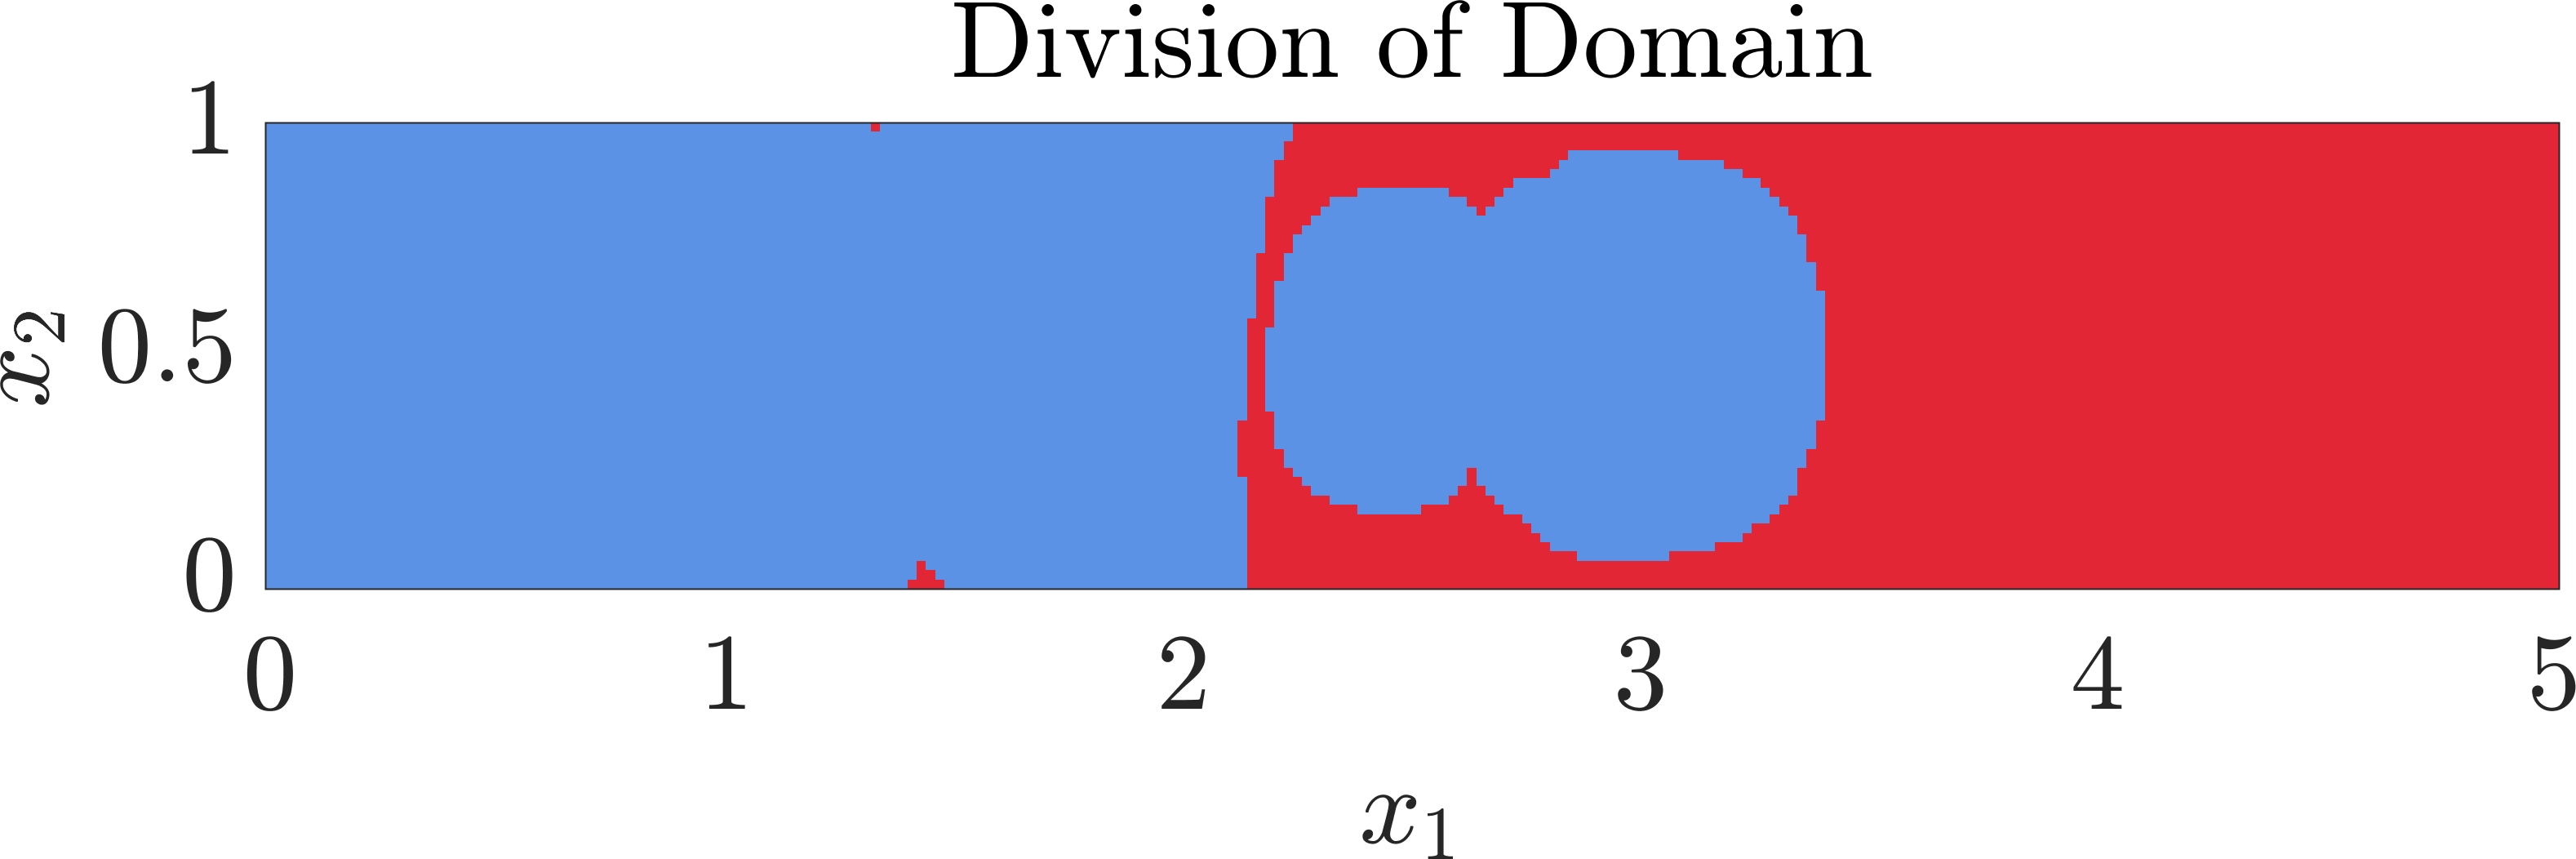
\includegraphics[width=0.46\textwidth]{svf/cd_cdr_MF06_divvy.jpeg}
  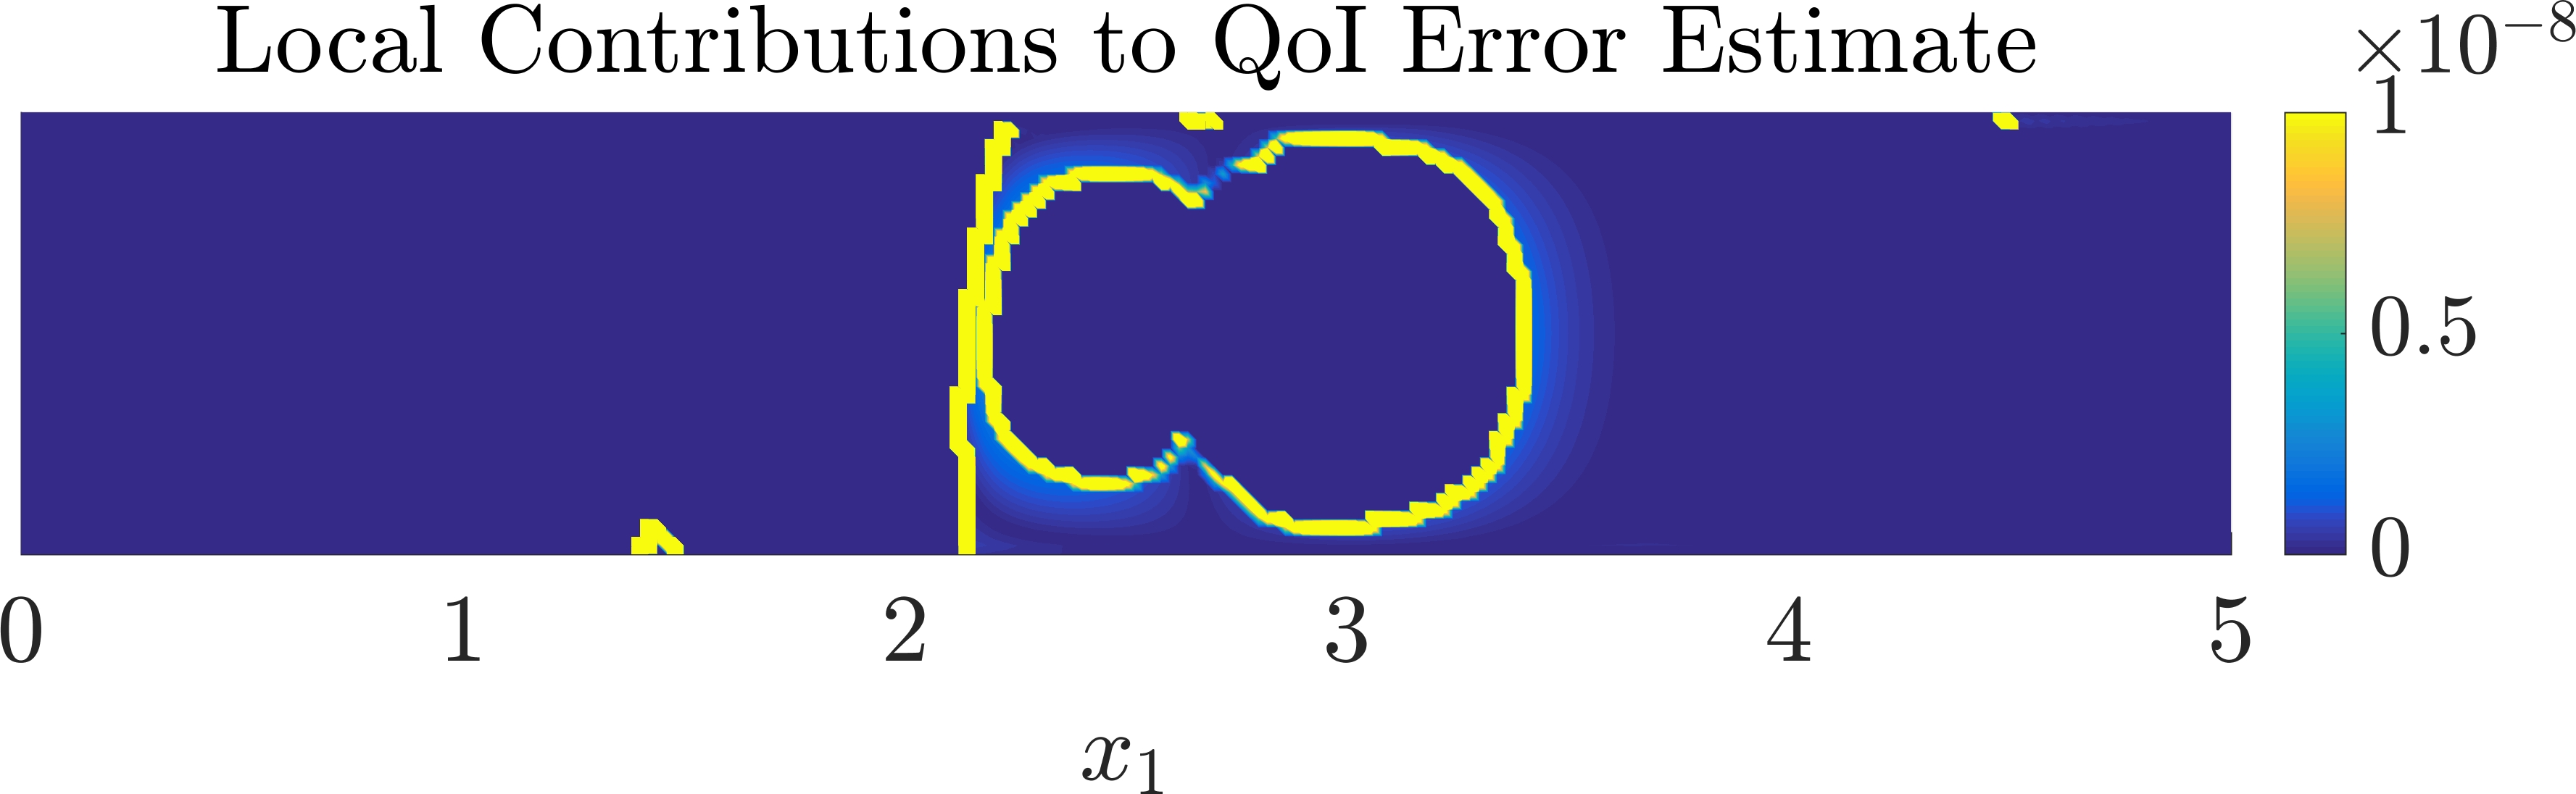
\includegraphics[width=0.49\textwidth]{svf/err_breakdown_MF06.jpeg}
}
\caption{Left: Multi-fidelity refinement over the domain (low-fidelity constant-parameter model used in red portion, high-fidelity field-parameter model used in blue portion). Right: local error contributions. The (weighted) residual, and thus the local error contribution, tends to spike sharply at the interface between the low- and high-fidelity regions; the color range is truncated to make the error distribution visible elsewhere in the domain.}
\label{fig:svfRef}
\end{figure}
%
Comparing to \Cref{fig:baseRef}, we see that in this case the local error contribution is not as greatly concentrated around the QoI region and the nearest observation location; here, all three observation locations and the QoI region have associated regions of sufficiently similar high local error that all are refined in the first iteration. This reflects the global nature of the differences between the low- and high-fidelity models. 

The corresponding true and estimated absolute errors in the QoI are shown in \Cref{fig:svfErr}.
%
\begin{figure}[htbp]
\centering
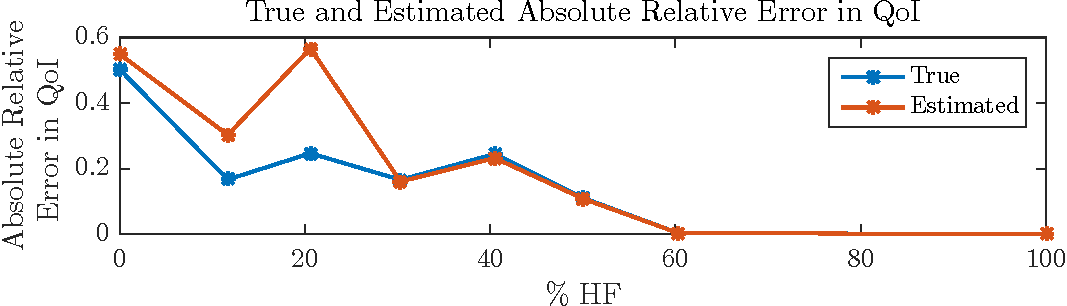
\includegraphics[width=0.8\textwidth]{svf/err_est.pdf}
\caption{True and estimated absolute relative error in QoI, plotted as a function of the percentage area of the domain in which the high-fidelity field-parameter model is used.}
\label{fig:svfErr}
\end{figure}
%
In this case, we see that we must use the high-fidelity model in most of the domain in order to get an accurate QoI. The adaptive algorithm requires us to use the field representation of the high-fidelity model in much of the left half of the domain; this reflects the topology of the inferred parameter field in the high-fidelity inverse problem, which is only relatively constant towards the right portion of the domain. We also see that in this case, in contrast to the example in \Cref{sec:cdvcdrBaseRef}, increasing the proportion of the domain in which the high-fidelity model is used does not monotonically decrease the error in the QoI.

%------------------------------------------------------------------------------------------------------------------------%
\subsection{Combining Meshes and Physics in 3D} \label{sec:diffvcdr3D}
%------------------------------------------------------------------------------------------------------------------------%

In the previous examples, although the low- and high-fidelity models are sufficiently different to illustrate the behavior of \Cref{alg:refSeries}, they are both simple enough and similar enough that using \Cref{alg:refSeries} saves little, if any, computational effort. In this section, we consider a pair of models that differ in both the physics included and the mesh resolution, and we demonstrate computational savings using the multi-fidelity approach. In \Cref{sec:setup3D_diffmesh} we describe the setup of the models and their inverse problems, and in \Cref{sec:ref3D_diffmesh} we describe the results of applying \Cref{alg:refSeries} to this pair of models.

%------------------------------------------------------------%
\subsubsection{Problem Setup} \label{sec:setup3D_diffmesh}
%------------------------------------------------------------%

The two models share a box domain $\Omega(x_1,x_2,x_3)$ which is $2300$m, $1650$m, and $100$m long in the $x_1$, $x_2$, and $x_3$ directions, respectively. We will refer to the positive and negative directions in $x_1$ as ``east" and ``west", respectively. The high-fidelity model is a single-species convection-diffusion-reaction equation with a nonlinear reaction term, described by
%
\begin{subequations}
\label{eq:cdvcdrHF3D}
\begin{align}
\nabla\cdot(n\vec{V}u - nD\nabla u) + k_ru^2 = f(q) \quad &\text{in } \Omega, \label{eq:HFeq3D}\\
u = 0 \quad &\text{on } \partial \Omega_{west}, \\
\frac{\partial u}{\partial n} = 0 \quad &\text{on }\partial\Omega_{east}, \\
\hat{n}\cdot(n\vec{V}u - nD\nabla u) = 0 \quad &\text{on }\partial\Omega\backslash(\partial\Omega_{east}\cup\partial\Omega_{west}),
\end{align}
\end{subequations}
%
where the state $u$ is the mass-fraction (in parts-per-billion) of some contaminant species and $f(q)$ is a source/sink field. The velocity field is a constant $\vec{V}=(2.1,0,0)$ m/day. Given this velocity field and letting the molecular diffusion be negligible, we follow \cite{Vestedetal93} to express the (diagonal) dispersion tensor $D$ as $D_{11}=\alpha_{LH}V_1$, $D_{22}=\alpha_{TH}V_1$, and $D_{33}=\alpha_{TV}V_1$, where $\alpha_{LH}=100$m, $\alpha_{TH}=40$m, and $\alpha_{TV}=4$m are the longitudinal horizontal, transverse horizontal, and transverse vertical dispersivities, respectively; the dispersivity values were drawn from within the range of observed values in various porous media \cite{Davis86}. We have porosity $n=0.1$. The reaction coefficient is $k_r=4.2\cdot10^{-4}$ 1/day, chosen from within the wide range of reaction-rate coefficients for second-order reactions. Although the reaction term $k_ru^2$ does not correspond to any particular reaction of any particular species, we note that, in addition to second-order elementary reactions, a quadratic reaction term can appear in models of dissolution/precipitation processes in porous media \cite{Aha97} and biochemical degradation of petroleum hydrocarbons in soils \cite{Jack94}.

The low-fidelity model,
%
\begin{equation}
\nabla\cdot(- nk_d\nabla u) = f(q) \quad \text{in } \Omega, \label{eq:LFeq3D}
\end{equation}
%
differs in the removal of the reaction and convection terms and the anisotropy of the dispersion tensor; the dispersion tensor $D$ is replaced with a scalar $k_d=D_{11}$. The boundary conditions remain unchanged. As in the previous examples in \Cref{sec:cdvcdr}, the mixed-fidelity models are formed by dividing the domain into complementary subdomains $\Omega_{HF}$ and $\Omega_{LF}$, where \Cref{eq:HFeq3D,eq:LFeq3D} are solved, respectively. The QoI we wish to calculate is the integral of the state over a region $\Omega_I$.

The unknown parameters we wish to infer correspond to the source term $f(q)=q$; we impose $f(q)=q=0$ on the boundary $\partial\Omega$. Synthetic observations at 18 points in the domain are generated by running the high-fidelity model on a finer mesh. The locations of the observations as well as the QoI region $\Omega_I$ are shown in \Cref{fig:setup3D}. We set the regularization term in \Cref{eq:invOpt_obj} to be $R(q)=\frac{\beta}{2}\int_\Omega \|\nabla f(q)\|_2^2\:\textrm{d}V$.
%
\begin{figure}[htbp]
\centering
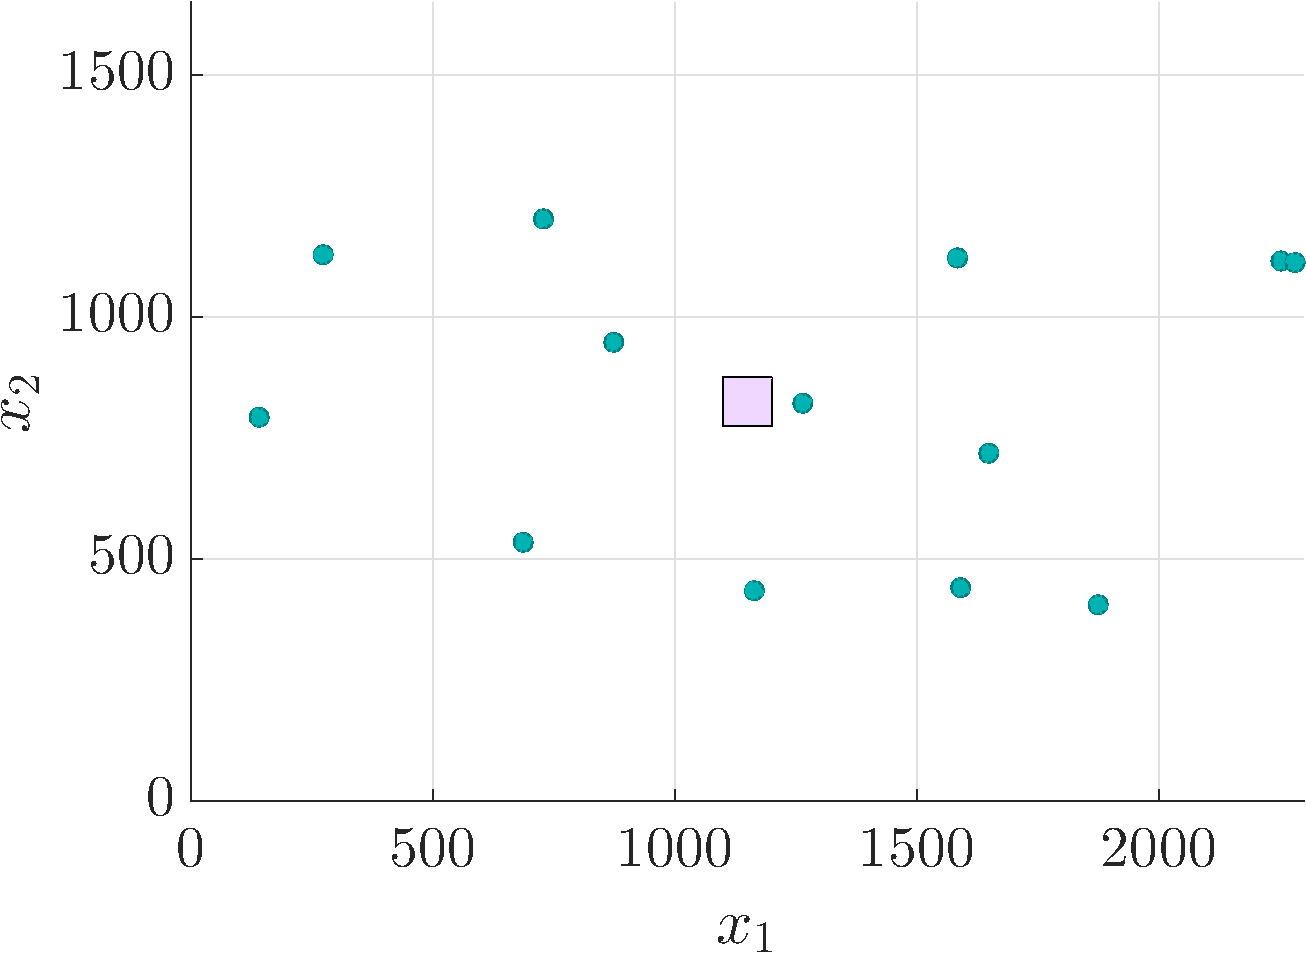
\includegraphics[width=0.4\textwidth]{series3D/setup_aerial_nolegend.pdf} \hfill
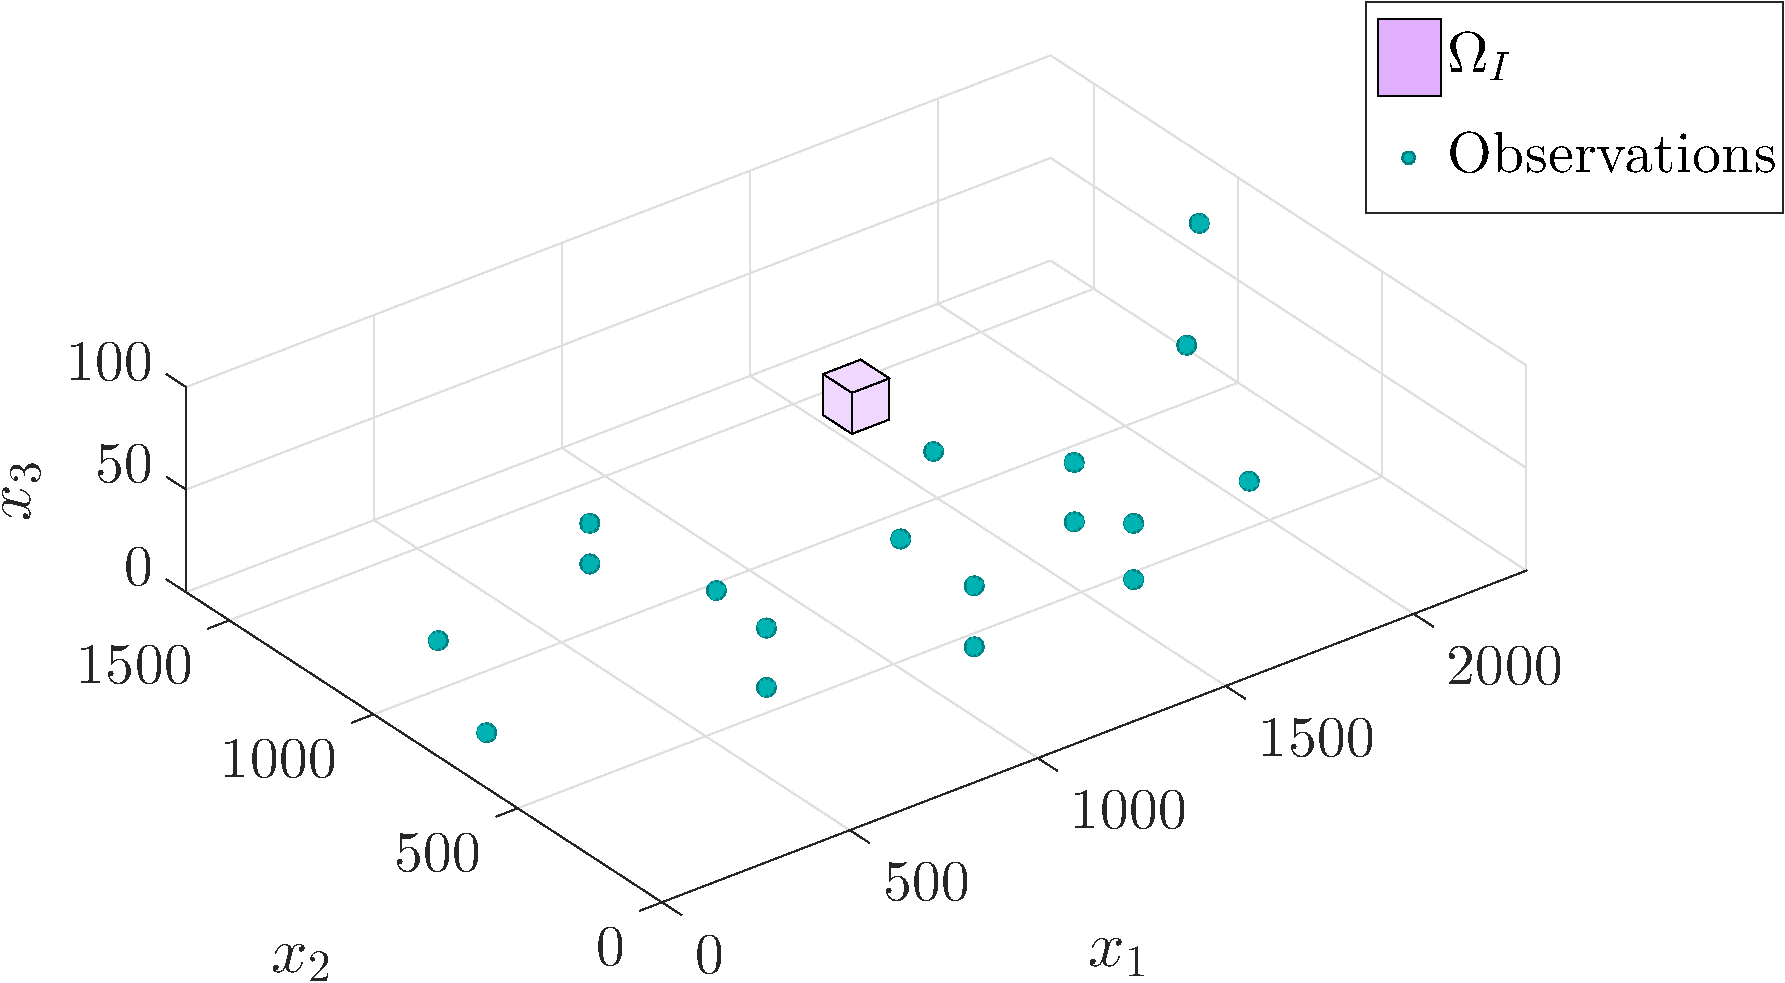
\includegraphics[width=0.55\textwidth]{series3D/setup_3view.pdf} \\
\vspace{\baselineskip}
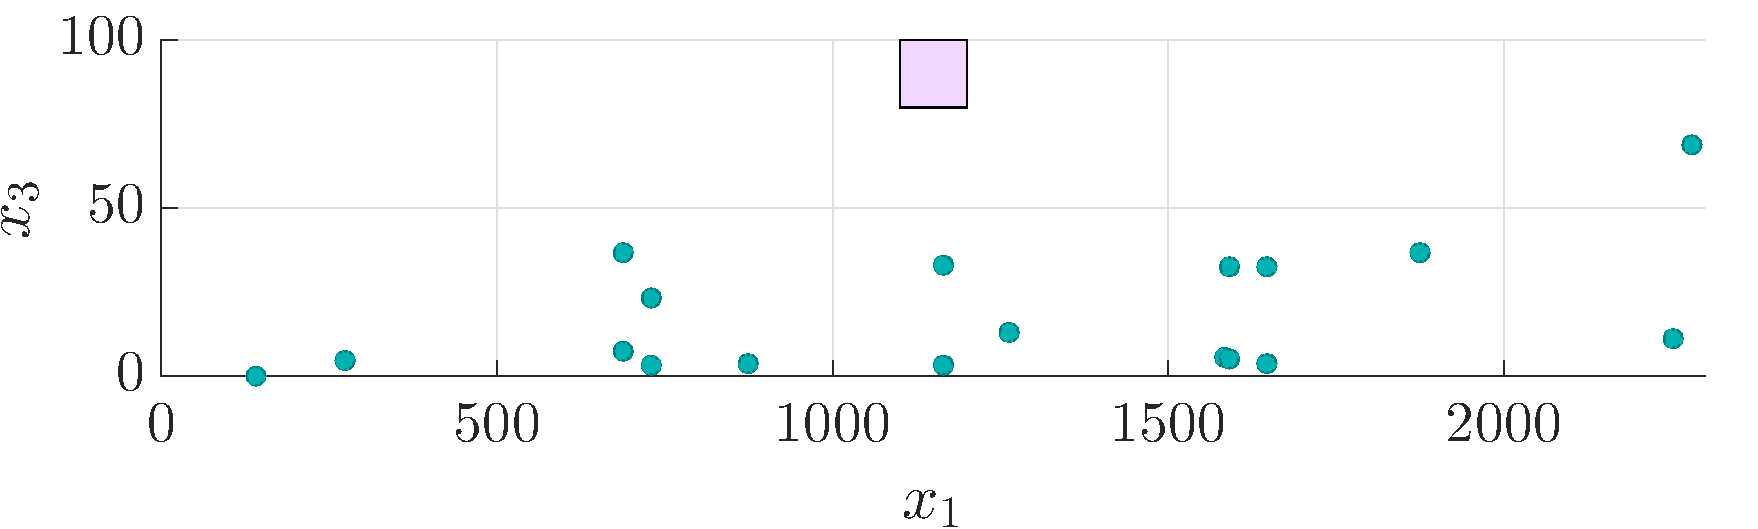
\includegraphics[width=0.6\textwidth]{series3D/setup_side_view.pdf}
\caption{Three views of the locations of the observations and the QoI region.}
\label{fig:setup3D}
\end{figure}
%

We use a FEM with a continuous Galerkin formulation and Lagrange elements. The lack of a convection term allows the low-fidelity model to be solved on a coarser mesh. For the high-fidelity model, the domain is discretized by 32, 64, and 32 elements along the $x_1$, $x_2$, and $x_3$ directions, respectively; for the low-fidelity model, the domain is discretized by 16, 32, and 16 elements along the $x_1$, $x_2$, and $x_3$ directions, respectively. The cell P\'{e}clet number is less than one and so stabilization is not required.

%------------------------------------------------------------%
\subsubsection{Adaptive Model Refinement Results} \label{sec:ref3D_diffmesh}
%------------------------------------------------------------%

We now present the results of solving the inference problem using \Cref{alg:refSeries}, with a relative error tolerance of $0.1\%$. At each iteration, we choose the $2\%$ of the basis functions with the largest error for model refinement; since each linear Lagrange basis function has eight elements in its support, the number of additional elements marked for refinement in each iteration is usually greater than for the 2D examples. All simulations are run on a single processor; we use the default nonlinear solver in \texttt{libMesh} \cite{libMeshPaper} (Newton's method with Brent line-search), and linear solves are performed using PETSc's \cite{petsc-user-ref} GMRES solver, preconditioned by incomplete factorization.

\Cref{tab:ref3D_diffmesh} shows the error at the end of each adaptive iteration. Each iteration of the adaptive algorithm uses the solution of the previous iteration as its initial guess. The number of degrees of freedom of each of the primary (and, if applicable, auxiliary) variables at each iteration is also given; the supplementary adjoint is solved on the high-fidelity mesh and thus each of its variables has the same number of degrees of freedom as each of the primary variables in the high-fidelity inverse problem. The high-fidelity inverse problem does not converge when the low-fidelity solution is used as an initial guess. Instead, we solve the inverse problem for an intermediate model
%
\begin{equation}
\nabla\cdot(n\vec{V}u - nD\nabla u) + k_ru^2 = f(q)
\end{equation}
%
and use the solution as an initial guess for the high-fidelity problem; equivalently, we use two steps of natural continuation on the reaction parameter: $k_r=0$, then $k_r=4.2\cdot10^{-4}$.
%
\begin{table}[htbp]
\label{tab:ref3D_diffmesh}
\centering
\begin{tabular}{|c|c|c|c|c|c|c|c|c|}
\hline
\multirow{2}{*}{Case} & \multirow{2}{*}{$\%$HF} & \multirow{2}{*}{DOFs} & \multirow{2}{*}{QoI} & Error & Error & $\%$ Relative \\
& & & & (Estimated) & (Actual) & Error (Actual)  \\ \hline
LF   & 0    & 9537  & 168710 & -16463 & -85663 & -103    \\
MF01 & 5.2  & 13417 & 167366 & -7207  & -84319 & -102    \\
MF02 & 11.4 & 17895 & 89777  & -6208  & -6730  & -8.10   \\
MF03 & 16.3 & 21001 & 85880  & -2473  & -2833  & -3.41   \\
MF04 & 22.0 & 24528 & 83902  & -711   & -855   & -1.03   \\
MF05 & 27.7 & 27984 & 83119  & 32     & -72    & -0.087  \\
HF   & 100  & 70785 & 83047  & --     & --     & --    \\ \hline
\end{tabular}
\caption{Runtime and relative errors of adaptive algorithm iterations given relative error tolerance of $0.1\%$; relative errors are given with respect to the high-fidelity QoI estimate.}
\end{table}
%

We notice that, compared to the results in \Cref{fig:baseErr}, the error estimates for the low-fidelity and first mixed-fidelity models are far from the true errors. This can be attributed to the linearization about $\Psi_{LF}$ and $\Psi_{MF_{1}}$ instead of $\Psi_{HF}$ in solving the supplementary adjoints as well as the third-order term that is ignored in the error estimate; the large differences in the QoI for the LF and MF01 models compared to the high-fidelity QoI indicate that $\Psi_{LF}$ and $\Psi_{MF_{1}}$ are significantly different from $\Psi_{HF}$. Compared to the pair of models in \Cref{sec:cdvcdrSetup}, the low- and high-fidelity models in this case are more dissimilar, even though in both \Cref{sec:cdvcdrSetup} and this case the nonlinear term in the high-fidelity model \Cref{eq:cdvcdrHF} and \Cref{eq:cdvcdrHF3D} is a quadratic reaction term. 

The multi-fidelity domain refinements for the five adaptive iterations are shown in \Cref{fig:divvy3D_diffmesh}. Similarly to the behavior seen in \Cref{sec:cdvcdrBaseRef}, the QoI region and the areas around some of the measurement points are first targeted for refinement, with those measurement points furthest downstream of the QoI being the last to receive refinement. We also see that the domain is refined completely in the $x_3$ direction first around the QoI region, reflecting the large difference in the high-fidelity dispersion tensor $D$ and the low-fidelity dispersion coefficient in the $x_3$ direction.
%
\begin{figure}[htbp]
\centering
\subfloat[MF$_1$ ($5.2\%$ HF)]{
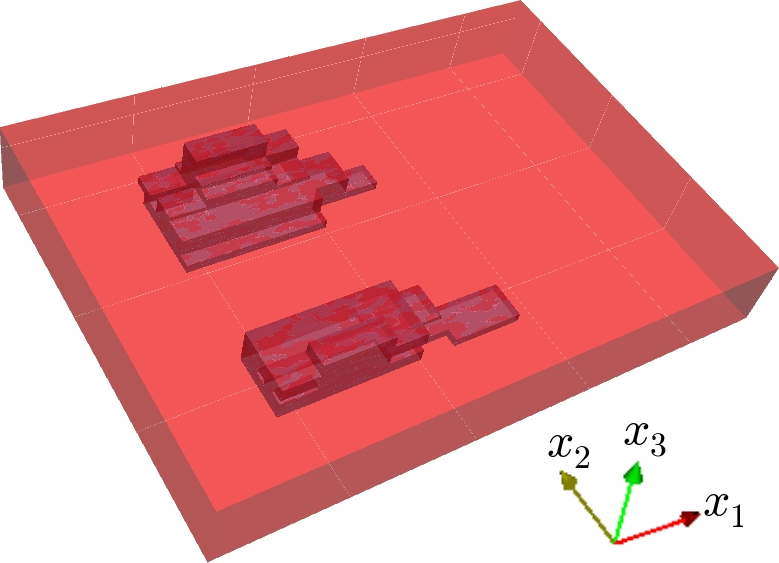
\includegraphics[width=0.31\textwidth]{series3D/run_diff_mesh/divvy1_whitebg_puff.jpeg}
}
\subfloat[MF$_2$ ($11.4\%$ HF)]{
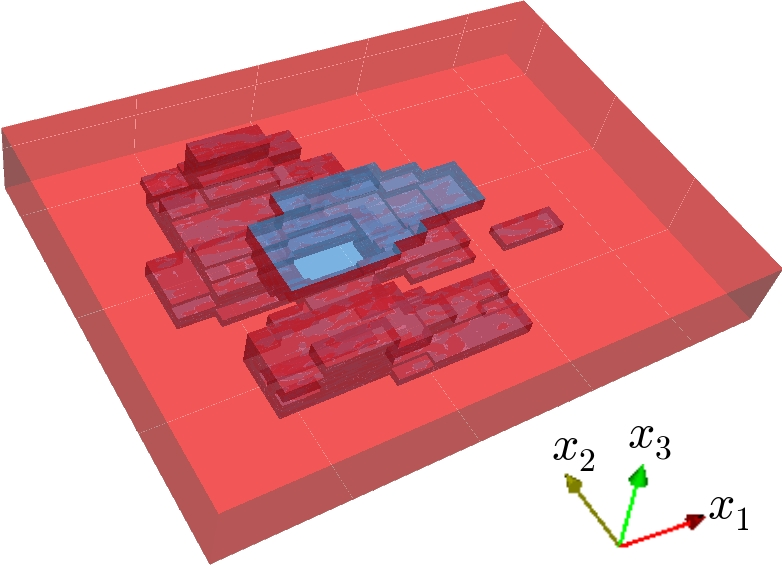
\includegraphics[width=0.31\textwidth]{series3D/run_diff_mesh/divvy2_whitebg_puff.jpeg}
}
\subfloat[MF$_3$ ($16.3\%$ HF)]{
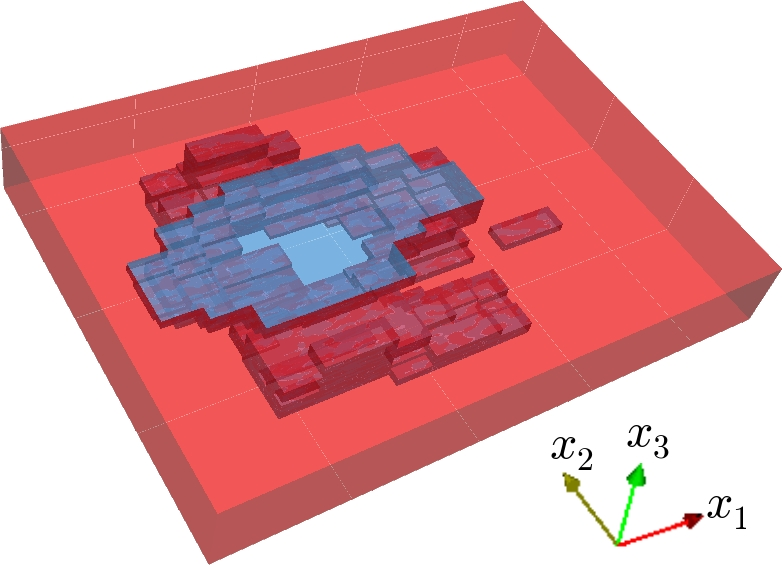
\includegraphics[width=0.31\textwidth]{series3D/run_diff_mesh/divvy3_whitebg_puff.jpeg}
} \\
\subfloat[MF$_4$ ($22.0\%$ HF)]{
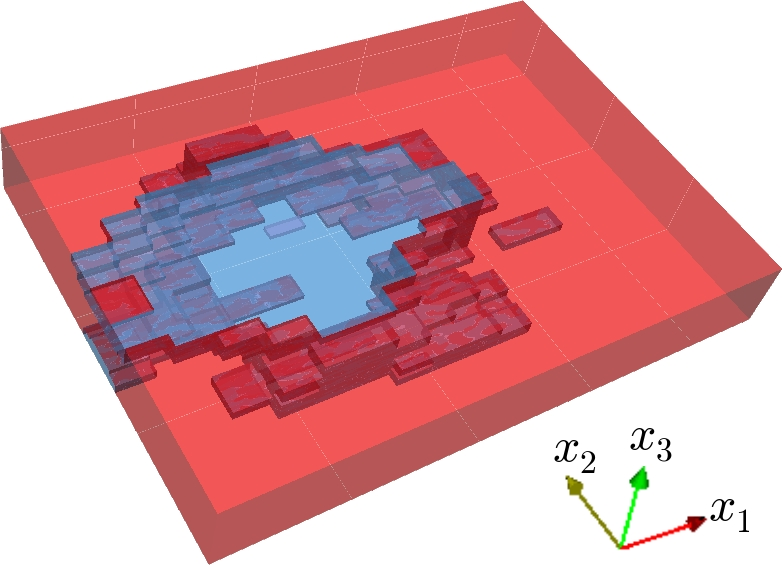
\includegraphics[width=0.31\textwidth]{series3D/run_diff_mesh/divvy4_whitebg_puff.jpeg}
}
\subfloat[MF$_5$ ($27.7\%$ HF)]{
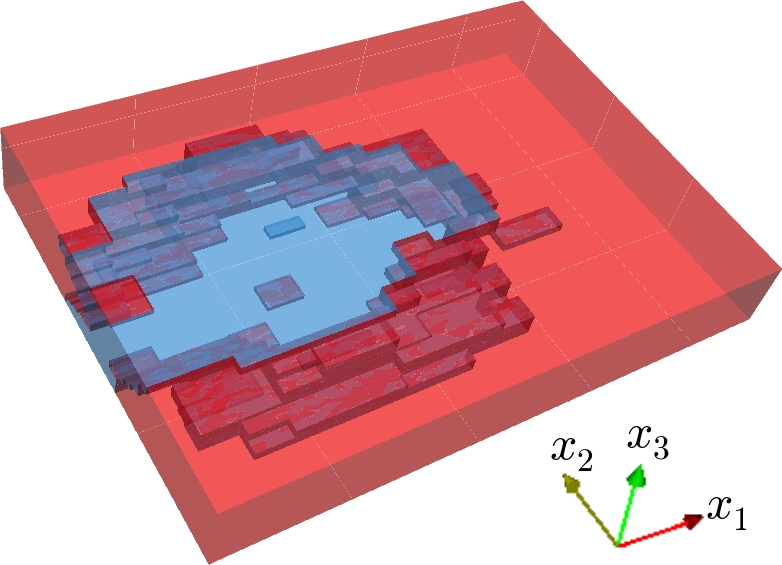
\includegraphics[width=0.31\textwidth]{series3D/run_diff_mesh/divvy5_whitebg_puff.jpeg}
}
\caption{Domain division for mixed-fidelity models: low-fidelity convection-diffusion model used in red portion, high-fidelity convection-diffusion-reaction model used in blue portion (intermediate colors due to transparency indicate a mix of the two models along the line of sight); $x_3$ direction scaled for clarity.}
\label{fig:divvy3D_diffmesh}
\end{figure}
%

In this case, although the mixed-fidelity models have fewer degrees of freedom than the high-fidelity model, it is faster to solve the high-fidelity inverse problem than to adaptively seek a mixed-fidelity model with a small QoI error, starting from the low-fidelity model. This can be attributed to multiple factors: the high-fidelity problem is mildly nonlinear and has a close initial guess that is a solution to a linear system (when $k_r=0$), and the supplementary adjoint is solved on the high-fidelity mesh. Generally, as the nonlinearity of the high-fidelity model increases, one would expect solving the high-fidelity inverse problem to require more time relative to using the adaptive algorithm. However, one can also consider an ``offline-online" setting, where the mixed-fidelity models are identified up-front by applying \Cref{alg:refSeries} to a set of representative observations $d^*$. Then when actual/new data are received, one can solve the inverse problem with the mixed-fidelity model and the new data, and, if desired, compute an updated error estimate for the QoI. The mixed-fidelity inverse problems are expected to require less time to solve than the high-fidelity inverse problems.

To illustrate this offline-online application, we generate ten sets of noisy observations to represent the actual data gained during the online phase; the noisy observations are generated by taking the observations used in the adaptive algorithm and adding Gaussian white noise with standard deviation of $\sigma=0.02$ (equivalent to, on average, $5\%$ of the observed values). We then solve the inverse problem using each of the mixed-fidelity models depicted in \Cref{tab:ref3D_diffmesh} and \Cref{fig:divvy3D_diffmesh} as well as the high-fidelity model. The low-fidelity inverse problem is first solved and used as an initial guess for the higher-fidelity problems; we note that although there is a linear model that is more similar to the high-fidelity model than the low-fidelity model (i.e., convection-diffusion with anisotropic diffusivity and $k_r=0$ on the high-fidelity mesh) and thus would serve as a better initial guess, its existence is specific to our particular choice of models. The auxiliary and supplementary adjoint variables use a zero initial guess.

\Cref{tab:ref3D_newdata_QoI_diffmesh} shows the average QoI values, error estimates and solution times for the (non)linear solves. \Cref{tab:ref3D_newdata_times_diffmesh} shows the times needed to solve the inverse problems and to solve for the additional variables needed to obtain an error estimate. For six of the ten datasets, the high-fidelity inverse problem does not converge given the low-fidelity solution as an initial guess; these are solved using the $k_r=0$ solution as an initial guess so that true QoI errors can be calculated. The average high-fidelity inverse problem solution time shown in \Cref{tab:ref3D_newdata_times_diffmesh} includes only those cases (four of ten) that converged with the low-fidelity initial guess.
%
\begin{table}
\label{tab:ref3D_newdata_QoI_diffmesh}
\centering
\begin{tabular}{|c|c|c|c|c|c|}
\hline
\multirow{2}{*}{Case} & \multirow{2}{*}{$\%$HF} & \multirow{2}{*}{QoI} & Error & Error & $\%$ Relative  \\
& & & (Estimated) & (Actual) & Error (Actual) \\ \hline
LF   & 0    & 166774 & --    & -84326 & -102.3 \\
MF01 & 5.2  & 164597 & 4347  & -82149 & -99.65  \\
MF02 & 11.4 & 88867  & -5921 & -6418  & -7.79  \\
MF03 & 16.3 & 85237  & -2414 & -2789  & -3.38  \\
MF04 & 22.0 & 83411  & -724  & -963   & -1.17  \\
MF05 & 27.7 & 82664  & -18   & -216   & -0.26 \\
HF   & 100  & 82500  & --    & --     & --  \\ \hline
\end{tabular}
\caption{Average QoI values and errors from solving inverse problem with mixed- and high-fidelity models and noisy data; relative errors are with respect to true high-fidelity QoI.}
\end{table}

%
\begin{table}
\caption{Average times to solve inverse problem and obtain error estimate with mixed- and high-fidelity models and noisy datasets.}
\label{tab:ref3D_newdata_times_diffmesh}
\centering
\begin{tabular}{ccc|c|c|c}
\cline{4-5}
 & & & \multicolumn{2}{|c|}{Error Estimation} & \\
\cline{1-6}
\multicolumn{1}{|c|}{\multirow{3}{*}{Case}} & \multicolumn{1}{|c|}{\multirow{3}{*}{DOFs}} & Inverse & Auxiliary & Supplementary & \multicolumn{1}{|c|}{Total} \\
\multicolumn{1}{|c|}{} & \multicolumn{1}{|c|}{} & Problem & Variables & Adjoint & \multicolumn{1}{|c|}{Solution}\\
\multicolumn{1}{|c|}{} & \multicolumn{1}{|c|}{} & Time (s) &  Time (s) & Time (s) & \multicolumn{1}{|c|}{Time (s)}\\
\cline{1-6}
\multicolumn{1}{|c|}{LF}    & \multicolumn{1}{|c|}{9537}   & 16   & --  & -- & \multicolumn{1}{|c|}{--} \\ \hline
\multicolumn{1}{|c|}{MF01}  & \multicolumn{1}{|c|}{13147}  & 185  & 107 & 235 & \multicolumn{1}{|c|}{526} \\ \hline
\multicolumn{1}{|c|}{MF02}  & \multicolumn{1}{|c|}{17895}  & 328  & 169 & 206 & \multicolumn{1}{|c|}{703} \\ \hline
\multicolumn{1}{|c|}{MF03}  & \multicolumn{1}{|c|}{21001}  & 435  & 202 & 185 & \multicolumn{1}{|c|}{821} \\ \hline
\multicolumn{1}{|c|}{MF04}  & \multicolumn{1}{|c|}{24528}  & 406  & 201 & 188 & \multicolumn{1}{|c|}{795} \\ \hline
\multicolumn{1}{|c|}{MF05}  & \multicolumn{1}{|c|}{27984}  & 498  & 263 & 198 & \multicolumn{1}{|c|}{959} \\ \hline
\multicolumn{1}{|c|}{HF}    & \multicolumn{1}{|c|}{70785}  & 1185 & --  & --  & \multicolumn{1}{|c|}{1185} \\ \hline
\end{tabular}
\end{table}
%
We see that the mixed-fidelity models, when applied to noisy datasets different to those with which they were generated, continue to perform well in achieving a small error in the QoI while limiting the use of the high-fidelity model to less than a third of the domain. Given the same initial guess, the mixed-fidelity inverse problems takes less time on average than the high-fidelity inverse problem to solve, and they converge consistently.


\section{Conclusion}\label{sec:conc}

We adaptively create mixed-fidelity models to solve goal-oriented inverse problems. The paper develops an error estimator that drives the adaptation, so as to minimize the error in the QoI calculated from the inferred parameters. We applied this method to pairs of low- and high-fidelity models of convection-diffusion-reaction phenomena. The results showed QoI estimates with a small relative error even when the high-fidelity model was used only in a small portion of the domain. In these cases, the localization of the error estimate also indicated regions of the domain that were important to the interactions between the observations and the QoI. A direction for extension of this work is to the case of the statistical inverse problem.  One way we could potentially apply this work to the statistical inverse problem is by reducing the parameter space that needs to be sampled. Such a direction is suggested by the results presented in \Cref{sec:diffvcdr3D}, where the mixed-fidelity model had significantly fewer degrees of freedom in its parameter field than the high-fidelity model, and thus a smaller parameter space. One could explore creation of an alternative statistical inverse problem that, by utilizing a mixed-fidelity model with fewer degrees of freedom in its parameter field, requires exploration of a small parameter space with minimal compromise in the predictive posterior.

Another potential approach would be to extend our method to the creation of mixed-fidelity models that are used as surrogates; these surrogate models can be evaluated in place of the high-fidelity model, thus decoupling the number of expensive forward evaluations of the high-fidelity model needed from the number of posterior parameter distribution samples that is desired \cite{Con14}. In such a case, the cost of creating the mixed-fidelity model would be amortized over a large number of posterior samples using the cheaper mixed-fidelity model in place of the high-fidelity model.

\section*{Acknowledgements}

This work was supported by the U.S. Department of Energy Office of Science, Office of Advanced Scientific
Computing Research, Applied Mathematics program under Award Number DE-FC02-13ER26129/DE-SC0009297 as part of the
DiaMonD Multifaceted Mathematics Integrated Capability Center.


%\nolinenumbers

\section*{References}
%\bibliographystyle{plain}
\bibliographystyle{elsarticle-harv} %this seems to get initials in bibliography, without doing name-year citation style as bst file claims?
\bibliography{masterBib}
\end{document}
